\section{Continuous Integration/Delivery}
\subsection{GitHub Actions}

allg. actions warum kosten
\subsubsection{Build IOS}
\setauthor{Martin Hausleitner}

\subsubsection{Build Android}

\subsection{Fastline}
\subsubsection{Build Number increment}
\subsection{Firebase App Distribution}

\section{Mobile Anwendung}
\subsection{Dateistruktur}
\setauthor{Martin Hausleitner}
In Flutter gibt es keine fixe Dateistruktur für eine App,
man kann seine Struktur also selbst überlegen und gestalten.
Im Folgenden beschreibe ich, wie wir unsere Dateistruktur
für eine Flutter-App aufgebaut haben.

In Flutter gibt es keine feste Dateistruktur, stattdessen kann man die Struktur der Dateien und Ordner selbst bestimmen. Für unser Flutter-Projekt haben wir uns für eine Struktur entschieden, die sich an bewährten Praktiken orientiert.

Die Dateistruktur sieht wie folgt aus:

\begin{itemize}
  \item \textbf{logic} - Hier befindet sich die Geschäftslogik der App, einschließlich der Firestore-Cloud-Funktionen und Repositories, die API-Aufrufe ausführen.
  \item \textbf{pages} - Hier werden Widgets entworfen, die jeweils eine Seite der App darstellen.
  \item \textbf{routes} - Hier werden die Routen definiert, die tiefere Links ermöglichen.
  \item \textbf{shared} - Hier werden UI-Widgets wie Buttons oder andere Widgets gespeichert, die oft wiederverwendet werden.
  \item \textbf{views} - Hier befinden sich Ansichten, die von mehreren Seiten der App verwendet werden können.
\end{itemize}

Im Nachhinein hätten wir die Dateistruktur anders gestaltet,
z.B. hätten wir das UI als eigenes Package definiert und die
pages und views besser unterteilt.

\subsection{State Management}
In Flutter gibt es verschiedene Möglichkeiten\cite{flutter-docs-interactive}\cite{flutter-state-management-blog}, um mit dem State Management umzugehen. State Management bezieht sich auf die Art und Weise, wie Daten innerhalb einer App verwaltet werden. In jeder App gibt es bestimmte Daten, die von verschiedenen Komponenten und Widgets verwendet werden und sich im Laufe der Zeit ändern können. State Management bezieht sich auf die Methoden, die verwendet werden, um diese Daten innerhalb der App zu verwalten und zu aktualisieren.
\setauthor{Martin Hausleitner}

\subsubsection{GetX}
\setauthor{Martin Hausleitner}

GetX verwendet ein reaktives Ansatz zur Verwaltung des Zustands, was bedeutet, dass Änderungen im Zustand automatisch die UI aktualisieren, ohne dass der Entwickler manuell Code schreiben muss, um diese Aktualisierungen durchzuführen. Dies spart viel Entwicklungszeit und macht es einfach, auf Benutzerinteraktionen zu reagieren.

Mit GetX können wir auch eine einheitliche Datenquelle haben, auf die alle Komponenten zugreifen können, was die Wartung und Erweiterung der Anwendung erleichtert. Darüber hinaus bietet GetX auch eine einfache Möglichkeit, Abhängigkeiten zu verwalten und Zustandsinformationen zwischen Bildschirmen zu teilen.

Insgesamt hat uns die Verwendung von GetX im Flutter-Framework sehr geholfen, eine effektive und skalierbare Anwendung zu erstellen, die auf die Bedürfnisse unserer Benutzer abgestimmt ist.
\setauthor{Sandin Habibovic}
getx controller service etc...


\subsection{Authentifizierung}
\setauthor{Sandin Habibovic}

\subsubsection{Anmelde Flow}
\setauthor{Sandin Habibovic}

Diagram
erklärung
screenshots
\subsubsection{Regestrierungs Flow}
\setauthor{Sandin Habibovic}


Diagram
erklärung
screenshots


\subsubsection{Firebase Authentifizierung}
\setauthor{Sandin Habibovic}

allg.


\subsection{Feed}
\setauthor{Sandin Habibovic}
Die Feed-Page ist die erste und wichtigste Anzeige auf der App. Hier werden alle aktuellen Beiträge und Updates von der Nachbarschaft angezeigt.

\subsection{Beiträge}
\setauthor{Sandin Habibovic}
Beiträge sind das Hauptkommunikationsmittel auf der App. Jedem Beitrag muss ein Titel, eine Beschreibung und eine Reichweite, unter der, der Beitrag sichtbar ist, angegeben werden. Weiters ist es möglich einem Beitrag ein Bild und Tags anzuhängen.

\subsubsection{Kategorien}
\setauthor{Sandin Habibovic}
Um Beiträge besser zuordnen zu können, muss der User den Beitrag vor dem Veröffentlichen in eine bestimmte Kategorie einteilen. Diese Kategorien ermöglichen es Usern, die Art Ihrer Anfrage ihm vorhinein besser zu spezifizieren und die Suche nach Beiträgen einer bestimmten Art zu vereinfachen. Bestimmte Kategorien werden weiters in Unterkategorien aufgeteilt, da diese ein zu weit gefächertes Genre an Anfragen umfassen.

Es existieren folgende Kategorien bzw. Unterkategorien:

\begin{compactitem}
  \item Mitteilung
  \begin{compactitem}
    \item Frage
    \item Appell
    \item Warnung
    \item Empfehlung
    \item Gefunden
  \end{compactitem}
  \item Suche
  \begin{compactitem}
    \item Hilfe
    \item Verloren
  \end{compactitem}
  \item Ausleihen
  \item Event
\end{compactitem}



Mitteilung:
Die Kategorie der Mitteilung dient dazu die Nachbarn über ein bestimmtes Ereignis oder Meldung zu informieren oder zu befragen.

Suche:
Die Kategorie der Suche dient dazu mit den Nachbarn im Falle einer Hilfesuche oder eines verloren gegangenen Objekts in Kontakt zu treten.

Ausleihen:
Die Kategorie des Ausleihens dient dazu die Nachbarn nach der Erlaubnis, sich ein bestimmtes Werkzeug oder Objekt ausborgen zu dürfen, zu bitten.

Event:
Die Kategorie des Events dient dazu die Nachbarn auf eine bestimmte Veranstaltung aufmerksam zu machen.


\subsubsection{Tags}
\setauthor{Sandin Habibovic}
Als Tag wird ein Schlüsselwort beschrieben, was man an ein Informationsgut anhängen kann, um es besser beschreiben zu können und/oder besser auffindbar zu machen. In der App werden Tags als eine Erweiterung der Kategorien verwendet, um es Usern zu ermöglichen Ihren Beitrag einem selbstdefinierten Typ zuzuordnen.

\subsubsection{Info}
\setauthor{Sandin Habibovic}
Jeder Beitrag hat eine eigene Sektion, wo wichtige Entscheidungsinformationen angegeben werden, wie der Stadtteil und die ungefähre Entfernung zum gegebenen Nachbarn und das Erstelldatum des Beitrags.

\subsubsection{Kommentare}
\setauthor{Sandin Habibovic}
Die Kommentarfunktion ermöglicht es den Usern unter einem Beitrag Ihre Meinung, Feedback oder sonstiges zu hinterlassen.

\subsubsection{Beitrag oder Kommentar Melden}
\setauthor{Sandin Habibovic}
Um auf unangebrachte Beiträge oder Kommentare schnell reagieren zu können, gibt es die Möglichkeit Beiträge oder Kommentare zu melden. Diese Meldungen werden auf Firestore gespeichert und können dann im Einzelnen überprüft werden. Fürs Melden muss ein Grund ausgewählt und eine genauere Beschreibung angegeben werden.
Gründe fürs Melden eines Beitrags oder Kommentars:

\begin{compactitem}
  \item Unangebrachter Inhalt
  \item Belästigung
  \item Betrug
  \item Spam
  \item Sonstiges
\end{compactitem}

\subsection{Filter}
\setauthor{Sandin Habibovic}
Der Filter bietet die Option die Beiträge nach bestimmten Kriterien zu filtern und die Suche nach bestimmten Beiträge zu vereinfachen. Der Filter unterteilt sich in einen Menüfilter und Hauptfilter.
Die Ansicht vom Menüfilter befindet sich direkt über den Beiträgen und ermöglicht eine schnelle Filterung nach einzig allein den Hauptkategorien.
Die Ansicht vom Hauptfilter taucht erst nach dem Antippen vom Filtersymbol auf und beinhaltet eine größere Auswahl an Filteroptionen. Darunter zählt neben dem Filtern nach Hauptkategorien auch die zusätzliche Möglichkeit genauer nach Unterkategorien zu suchen. Außerdem besteht auch die Option die Beiträge nach Datum oder Likes zu sortieren oder die Beiträge aufsteigend oder absteigend zu ordnen. Die wichtigste Filterkomponente ist der Range-Slider, womit die Beiträge nach der Reichweite gefiltert werden können, da die Entfernung zum Nachbarn eine der wichtigsten Entscheidungsfaktoren zum Antworten auf einem Beitrag ist.

\subsection{Suche}
\subsection{Typesense}
\subsection{Algolia}
diagram
\subsubsection{Firestore Sync}

\subsubsection{Algolia SDK}


\subsection{Chat}
package genommen warum
\subsubsection{Flyer Package}

\subsection{Profil}
\setauthor{Sandin Habibovic}
Die Profilanzeige ist die öffentliche Informationsstelle über den User. In dieser Anzeige werden als erster Eindruck der Name und das Profilbild vom User angezeigt. Genauere Informationen über den User können im Bereich Nutzerinfo gefunden werden. Darunter zählen:
\begin{compactitem}
  \item Geburtstag
  \item Beruf
  \item Bio
\end{compactitem}
Außerdem beinhaltet die Anzeige eine eigene Beitragssicht, wo alle Beiträge vom jeweiligen User eingesehen werden können.

\subsubsection{Profil Melden}
\setauthor{Sandin Habibovic}
Falls das Profil vom User unangebrachten Inhalt aufweist, besteht die Möglichkeit das Profil zu melden.

\subsection{Benachrichtigungen}
\setauthor{Sandin Habibovic}
Benachrichtigungen dienen dazu die Nachbarn über mögliche Hilfsbereitstellungen zu informieren, bevor der Kontakt überhaupt entsteht. Die Benachrichtigung zeigt den Nachbarn an, der in Kontakt treten möchte, und möglicherweise den Beitrag auf dem geantwortet wurde. Außerdem ist die Benachrichtigung mit einem „Annehmen“- und „Ablehnen“- Button ausgestattet, womit das Hilfsangebot angenommen oder abgelehnt werden kann.

\subsection{Einstellungen}
\setauthor{Sandin Habibovic}
Die Einstellungssicht der Anwendung bietet eine Reihe an nützlichen Funktionen, die dem User mehr Kontrolle über sein Konto geben.
Dazu gehört zu einem die Option, die Sprache der App umzustellen, um dem User zu ermöglichen, die Anwendung in der bevorzugten Sprache zu nutzen. Zum derzeitigen Stand kann die App sich in zwei Sprachen übersetzen lassen: Deutsch und Englisch.
Darüber hinaus können Benutzer auch entscheiden, ob sie Benachrichtigungen erhalten möchten oder nicht, und diese Einstellungen jederzeit ein- oder ausschalten. Diese Einstellungen bieten den Benutzern eine höhere Privatsphäre und Personalisierungsmöglichkeiten, um die Anwendung besser an ihre individuellen Bedürfnisse anzupassen.
Zu den weiteren Einstellungen gehört das Umändern der E-Mail oder des Passworts, um die Sicherheit des Kontos zu gewährleisten und unbefugten Zugriff zu verhindern.
Die letzte Funktion in der Einstellungssicht ist das Löschen des eigenen Kontos, womit alle Daten des Users gelöscht werden. Vor dem endgültigen Löschen des Kontos wird der User allerdings aufgefordert, seine Entscheidung zu bestätigen.

\subsection{Feedback}
\setauthor{Martin Hausleitner}
Im Zuge unserer Testphase suchen wir nach einer effizienten Methode, um Feedback zu sammeln. Um ein fundiertes Verständnis einer Fehlermeldung zu erlangen, erweist sich die Bereitstellung eines Screenshots als besonders nützlich. Daher haben wir uns nach Packages umgesehen, welche die Möglichkeit bieten, Screenshots zu erstellen und ergänzende Informationen als Kontext hinzuzufügen. Wir haben uns für das Package https://pub.dev/packages/feedback entschieden. Dieses Package gestattet dem Nutzer, einen Screenshot anzufertigen und Annotationen hinzuzufügen, bevor ein entsprechender Kontext in Textform eingefügt werden kann. Eine weitere praktische Funktion besteht darin, dass der Nutzer bei Bedarf noch einmal navigieren und den Screenshot wiederholen kann. Zur Initiierung dieses Feedback-Views haben wir das Package https://pub.dev/packages/shake genutzt, welches bei einer entsprechenden Bewegung des Mobilgeräts aktiviert wird. Wir haben uns bei dieser Funktion an anderen Anwendungen orientiert, die ähnliche Mechanismen für die Feedback-Erhebung nutzen.

Das von uns gewählte Vorgehen zur Analyse des Feedbacks erfolgt über die Trello-API, welche es uns ermöglicht, ein entsprechendes Dashboard zur Erfassung und Bearbeitung der Meldungen zu erstellen. Die erfassten Informationen, wie beispielsweise der Screenshot, der Text, das Datum und relevante Systeminformationen, dienen uns als Grundlage für eine weitere Auswertung und Fehlerbehebung. Trello erleichtert uns die Verwaltung des Feedbacks auf kostenlose Weise und stellt somit ein adäquates Instrument zur Unterstützung des Entwicklungsprozesses dar.


\section{UI/UX Design}
Das Design der Nachbarschafts-App war für das Team von hoher Bedeutung, weshalb der Designer Martin Hausleitner erheblichen Zeit- und Arbeitsaufwand aufwendete, um ein anspruchsvolles Design zu gestalten. Angesichts der Tatsache, dass die App ein breites Publikum ansprechen soll, einschließlich verschiedener Altersgruppen, war es von entscheidender Bedeutung sicherzustellen, dass die Benutzer die App einfach und intuitiv bedienen können. Um dieses Ziel zu erreichen, wurde eine klare Struktur und Navigation in das Design integriert, um den Benutzern eine einfache und effektive Nutzung der gewünschten Funktionen zu ermöglichen. Es wurde darauf geachtet, dass die Buttons gut erkennbar und mit aussagekräftigen Icons und verständlichen Beschriftungen versehen sind, um Verwirrung zu vermeiden. Weiterhin wurde das Design der Karten auf eine organische Weise gestaltet, um ein harmonisches und ästhetisches Gesamtbild zu erzeugen.
\setauthor{Martin Hausleitner}
\subsection{Inspiration}
Während des Designprozesses für die App wurden umfangreiche Recherchen im Bereich App-Design durchgeführt. Das Ziel war, die App so intuitiv wie möglich zu gestalten, um eine benutzerfreundliche Erfahrung sicherzustellen. Dabei wurden bekannte Social-Media-Apps wie \href{https://twitter.com/}{Twitter}, \href{https://www.instagram.com/}{Instagram} und \href{https://www.tiktok.com/}{TikTok} als Orientierung genutzt, da diese bereits erfolgreich auf dem Markt etabliert sind und von vielen Menschen vertraut genutzt werden.

Zusätzlich diente die erfolgreichste Nachbarschafts-App in Deutschland, \href{https://nebenan.de/}{Nebenan}, als Grundlage für die App-Entwicklung. Allerdings wurde festgestellt, dass ihre App sehr kompliziert aufgebaut und unübersichtlich ist. Daher wurde dies als Chance gesehen, um es besser zu machen.

Zur Entwicklung eines einfachen und schlichten Designs wurden Inspirationen von Websites wie \href{https://dribbble.com/}{Dribble} und \href{https://mobbin.design/}{Mobbin} genutzt. Insgesamt war die Recherche und Inspiration für das Design der App ein wichtiger Schritt, um sicherzustellen, dass Benutzer eine ansprechende und intuitive Erfahrung haben.

\subsection{Prototyping}
Das Team legte von Anfang an großen Wert auf eine exzellente
Benutzererfahrung, und daher war es ihnen klar, dass ein
Prototyp gestaltet werden musste. Das Prototyping hatte für
die Entwickler den großen Vorteil, dass sie beim
Programmieren in Flutter nicht mehr lange darüber nachdenken
mussten, wie Menüs oder Bildschirme gestaltet werden
sollten. Somit war es einfach für Teammitglieder, die nicht
mit Design vertraut waren, den Prototypen als Grundlage zu
nutzen, um ihre Umsetzung in Flutter zu gestalten. Der
Prototyp selbst war für den Designer Martin Hausleitner eine
Reise durch verschiedene Designer-Tools, die im folgenden
Absatz genauer behandelt werden.


\subsubsection{Framer}

Framer ist eine Software, die es Benutzern ermöglicht, schnell und einfach ansprechende Prototypen von mobilen Anwendungen und Websites zu erstellen. Das Tool wurde ursprünglich als Prototyping-Tool für Designer entwickelt, um Designs schnell zu testen und zu verfeinern, bevor sie in die Entwicklung übergehen.

Erfolgreiche Apps wie Spotify haben Framer im Rahmen ihres
Prototyping-Prozesses verwendet, um schnell und effizient
funktionierende App-Designs zu erstellen. Framer ist eine
schnelle und effiziente Möglichkeit, um Ideen in die Tat
umzusetzen, ohne sich durch langwierige Entwicklungsprozesse
zu quälen. Dies sind überzeugende Gründe für den Designer, den ersten Prototypen mit Framer zu gestalten.

\begin{figure}[h]
  \centering
  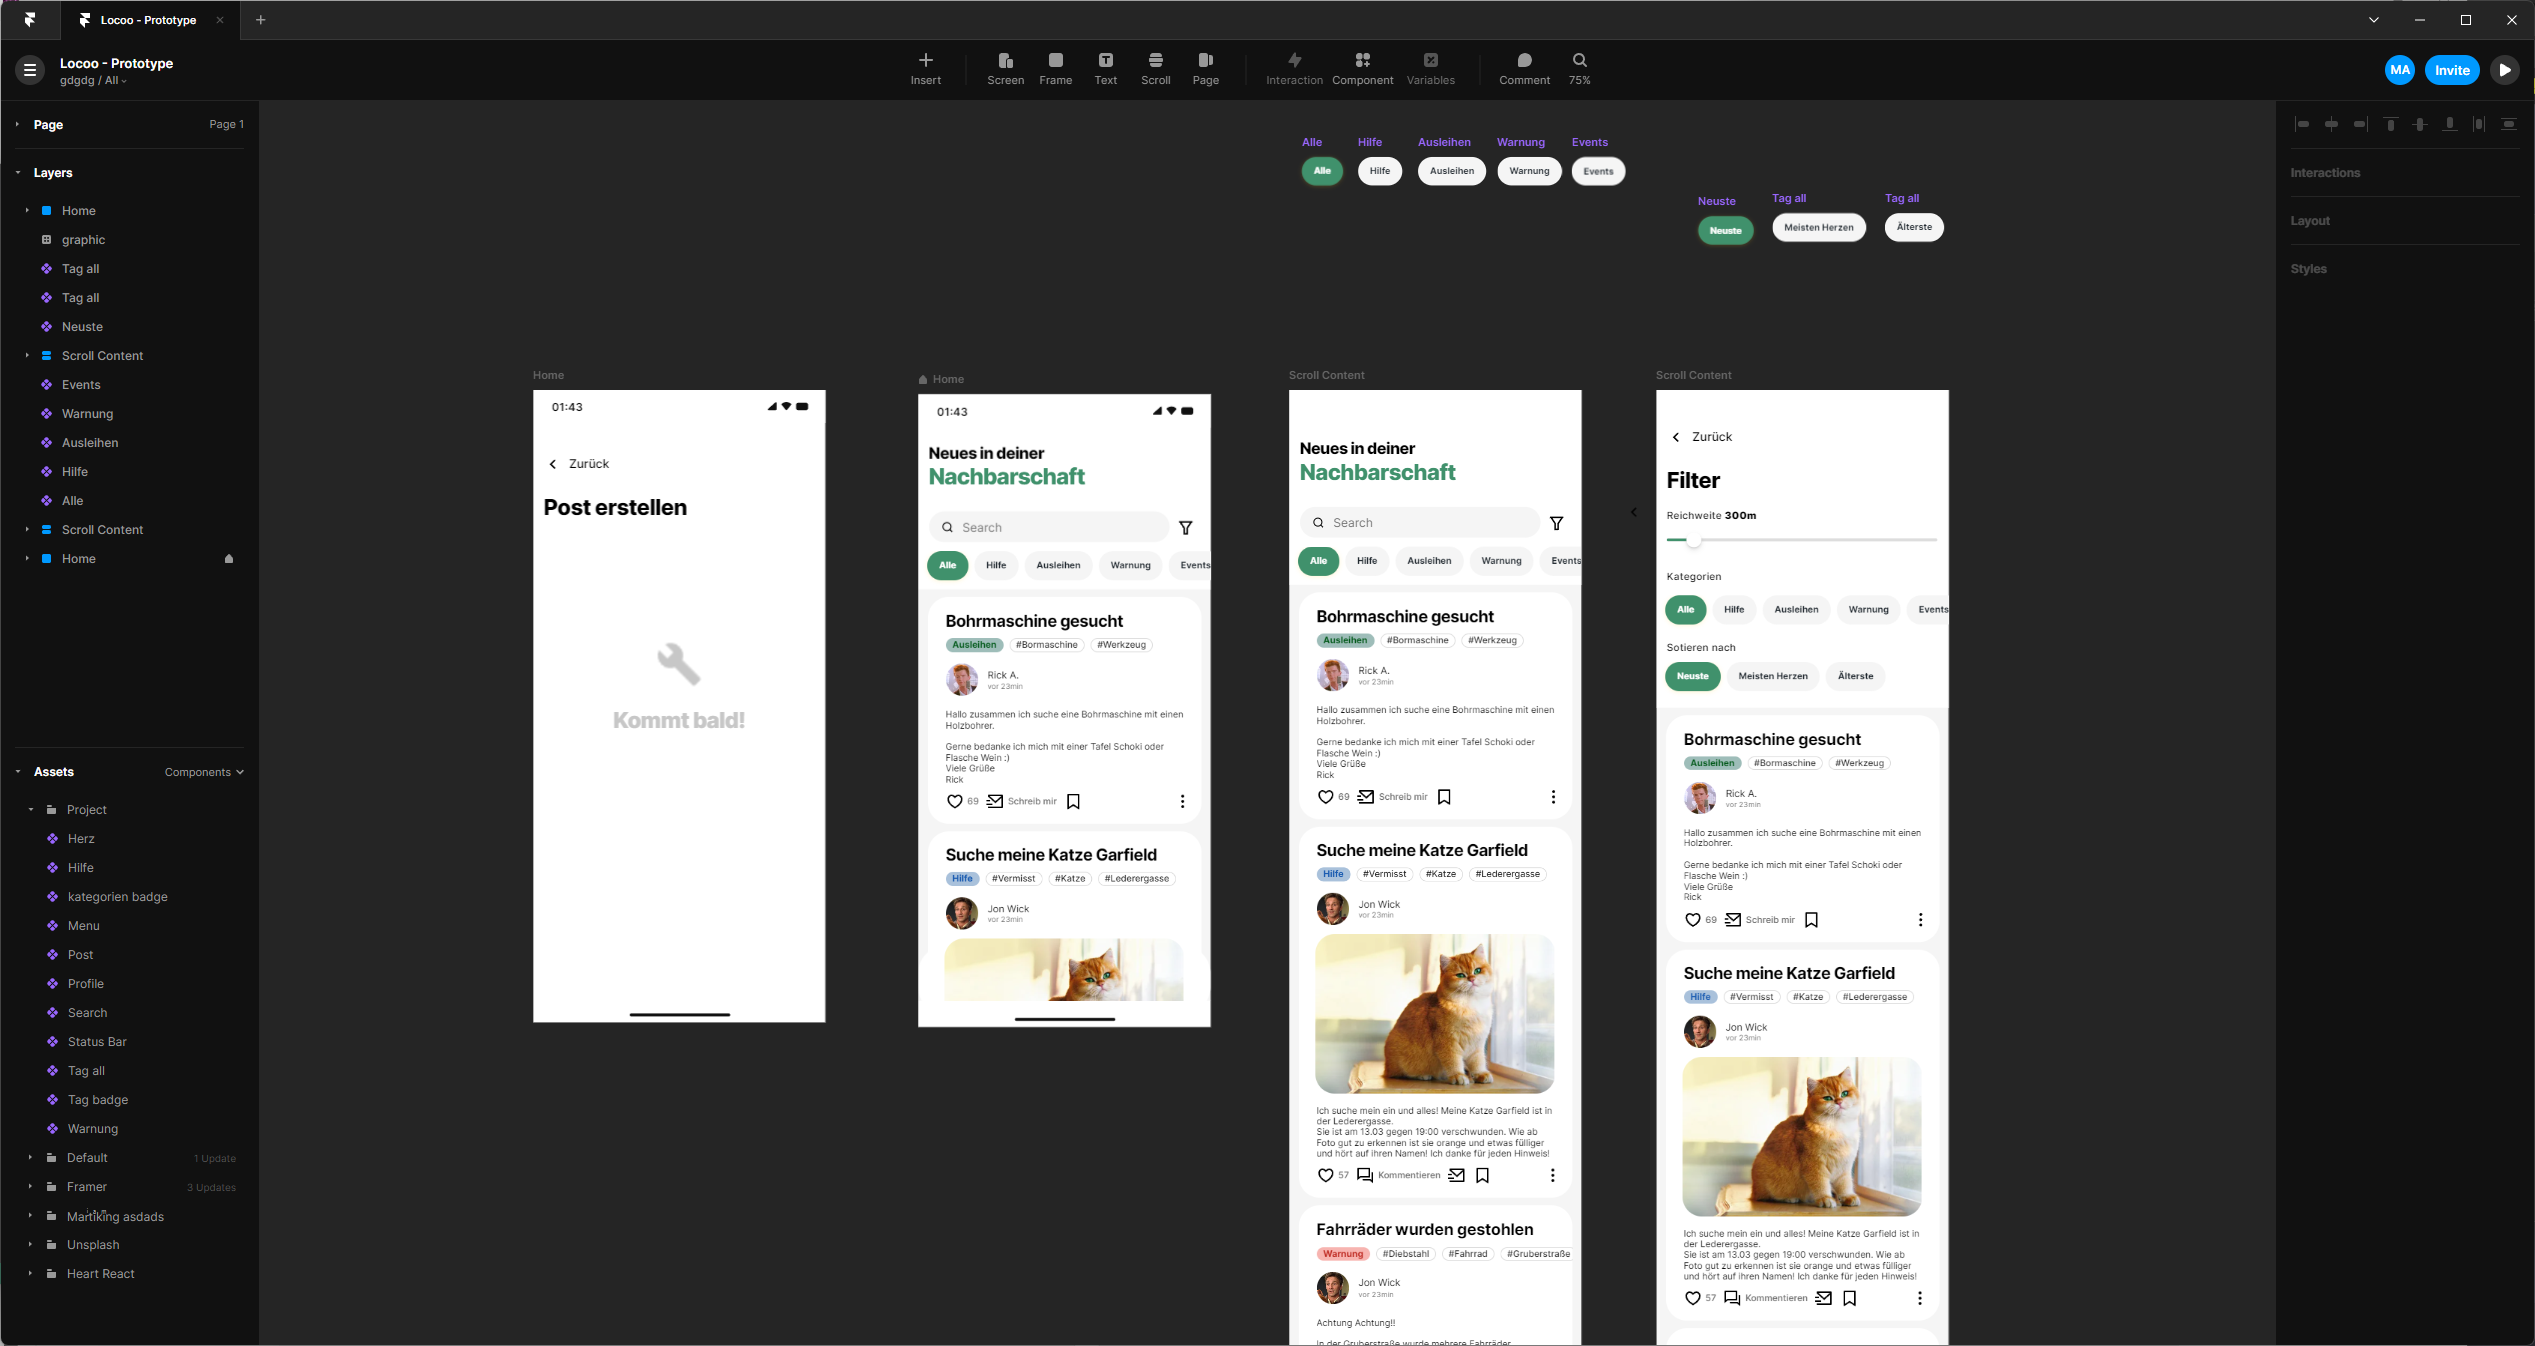
\includegraphics[width=1\textwidth]{pics/nochba-framer-prototype-screenshot.png}
  \caption{Nochba Prototyp in Framer}
  \label{fig:framer-prototype}
\end{figure}


Framer wurde während des Hackerthon Linz haCKt verwendet, um
den ersten Prototypen zu erstellen wie bei der man bei der
Abbildung \ref{fig:framer-prototype} erkennen kann. Die Wahl von Framer war
aufgrund seiner Geschwindigkeit und Effizienz in der
Erstellung von funktionsfähigen App-Designs und der
Erfahrung, die der Benutzer bereits mit dem Tool hatte,
getroffen worden.

Seit der Erstellung des ersten Prototyps hat sich das Geschäftsmodell von Framer jedoch geändert. Es ist jetzt ein Website-Baukasten, der es Benutzern ermöglicht, einfach und schnell ansprechende Websites zu erstellen, ohne Kenntnisse in der Webentwicklung zu benötigen. Obwohl es nun als Website-Baukasten fungiert, behält Framer immer noch einige seiner Kernfunktionen als Prototyping-Tool bei, was es zu einer guten Option für Designer und Entwickler macht, die schnell Prototypen erstellen möchten.

Insgesamt hat Framer gezeigt, dass es ein schnelles und effektives Tool ist, um Designideen in die Tat umzusetzen. Obwohl es nun als Website-Baukasten fungiert, ist es immer noch eine nützliche Option für Designer und Entwickler, die schnell und einfach Prototypen erstellen möchten.

\subsubsection{Adobe XD}
Bei der ersten Nutzung von Framer wurden zahlreiche Funktionen und Optionen entdeckt, was zunächst begeisterte. Doch mit der Zeit wurde erkannt, dass dies für das betreffende Projekt zu umfangreich war und somit nach einer einfacheren Lösung gesucht werden musste. Die Wahl fiel auf Adobe XD, da bereits jahrelange Erfahrung mit diesem Tool vorhanden war.

Trotz des geringeren Funktionsumfangs im Vergleich zu Framer
ist Adobe XD aufgrund seiner Benutzerfreundlichkeit und
Einfachheit ein ideales Werkzeug, um schnell Prototypen zu
erstellen. Alle Hauptscreens wurden fertiggestellt wie man
bei Abbildung \ref{fig:adobexd-prototyp} sehen kann, bevor
die Entwicklung mit Flutter begann. Die anderen wichtigen
Screens wurden später gestaltet, nachdem eine bessere
Kenntnis von Flutter erlangt wurde und es möglich war, den
Aufwand für die Umsetzung besser abzuschätzen.

\begin{figure}[h]
  \centering
  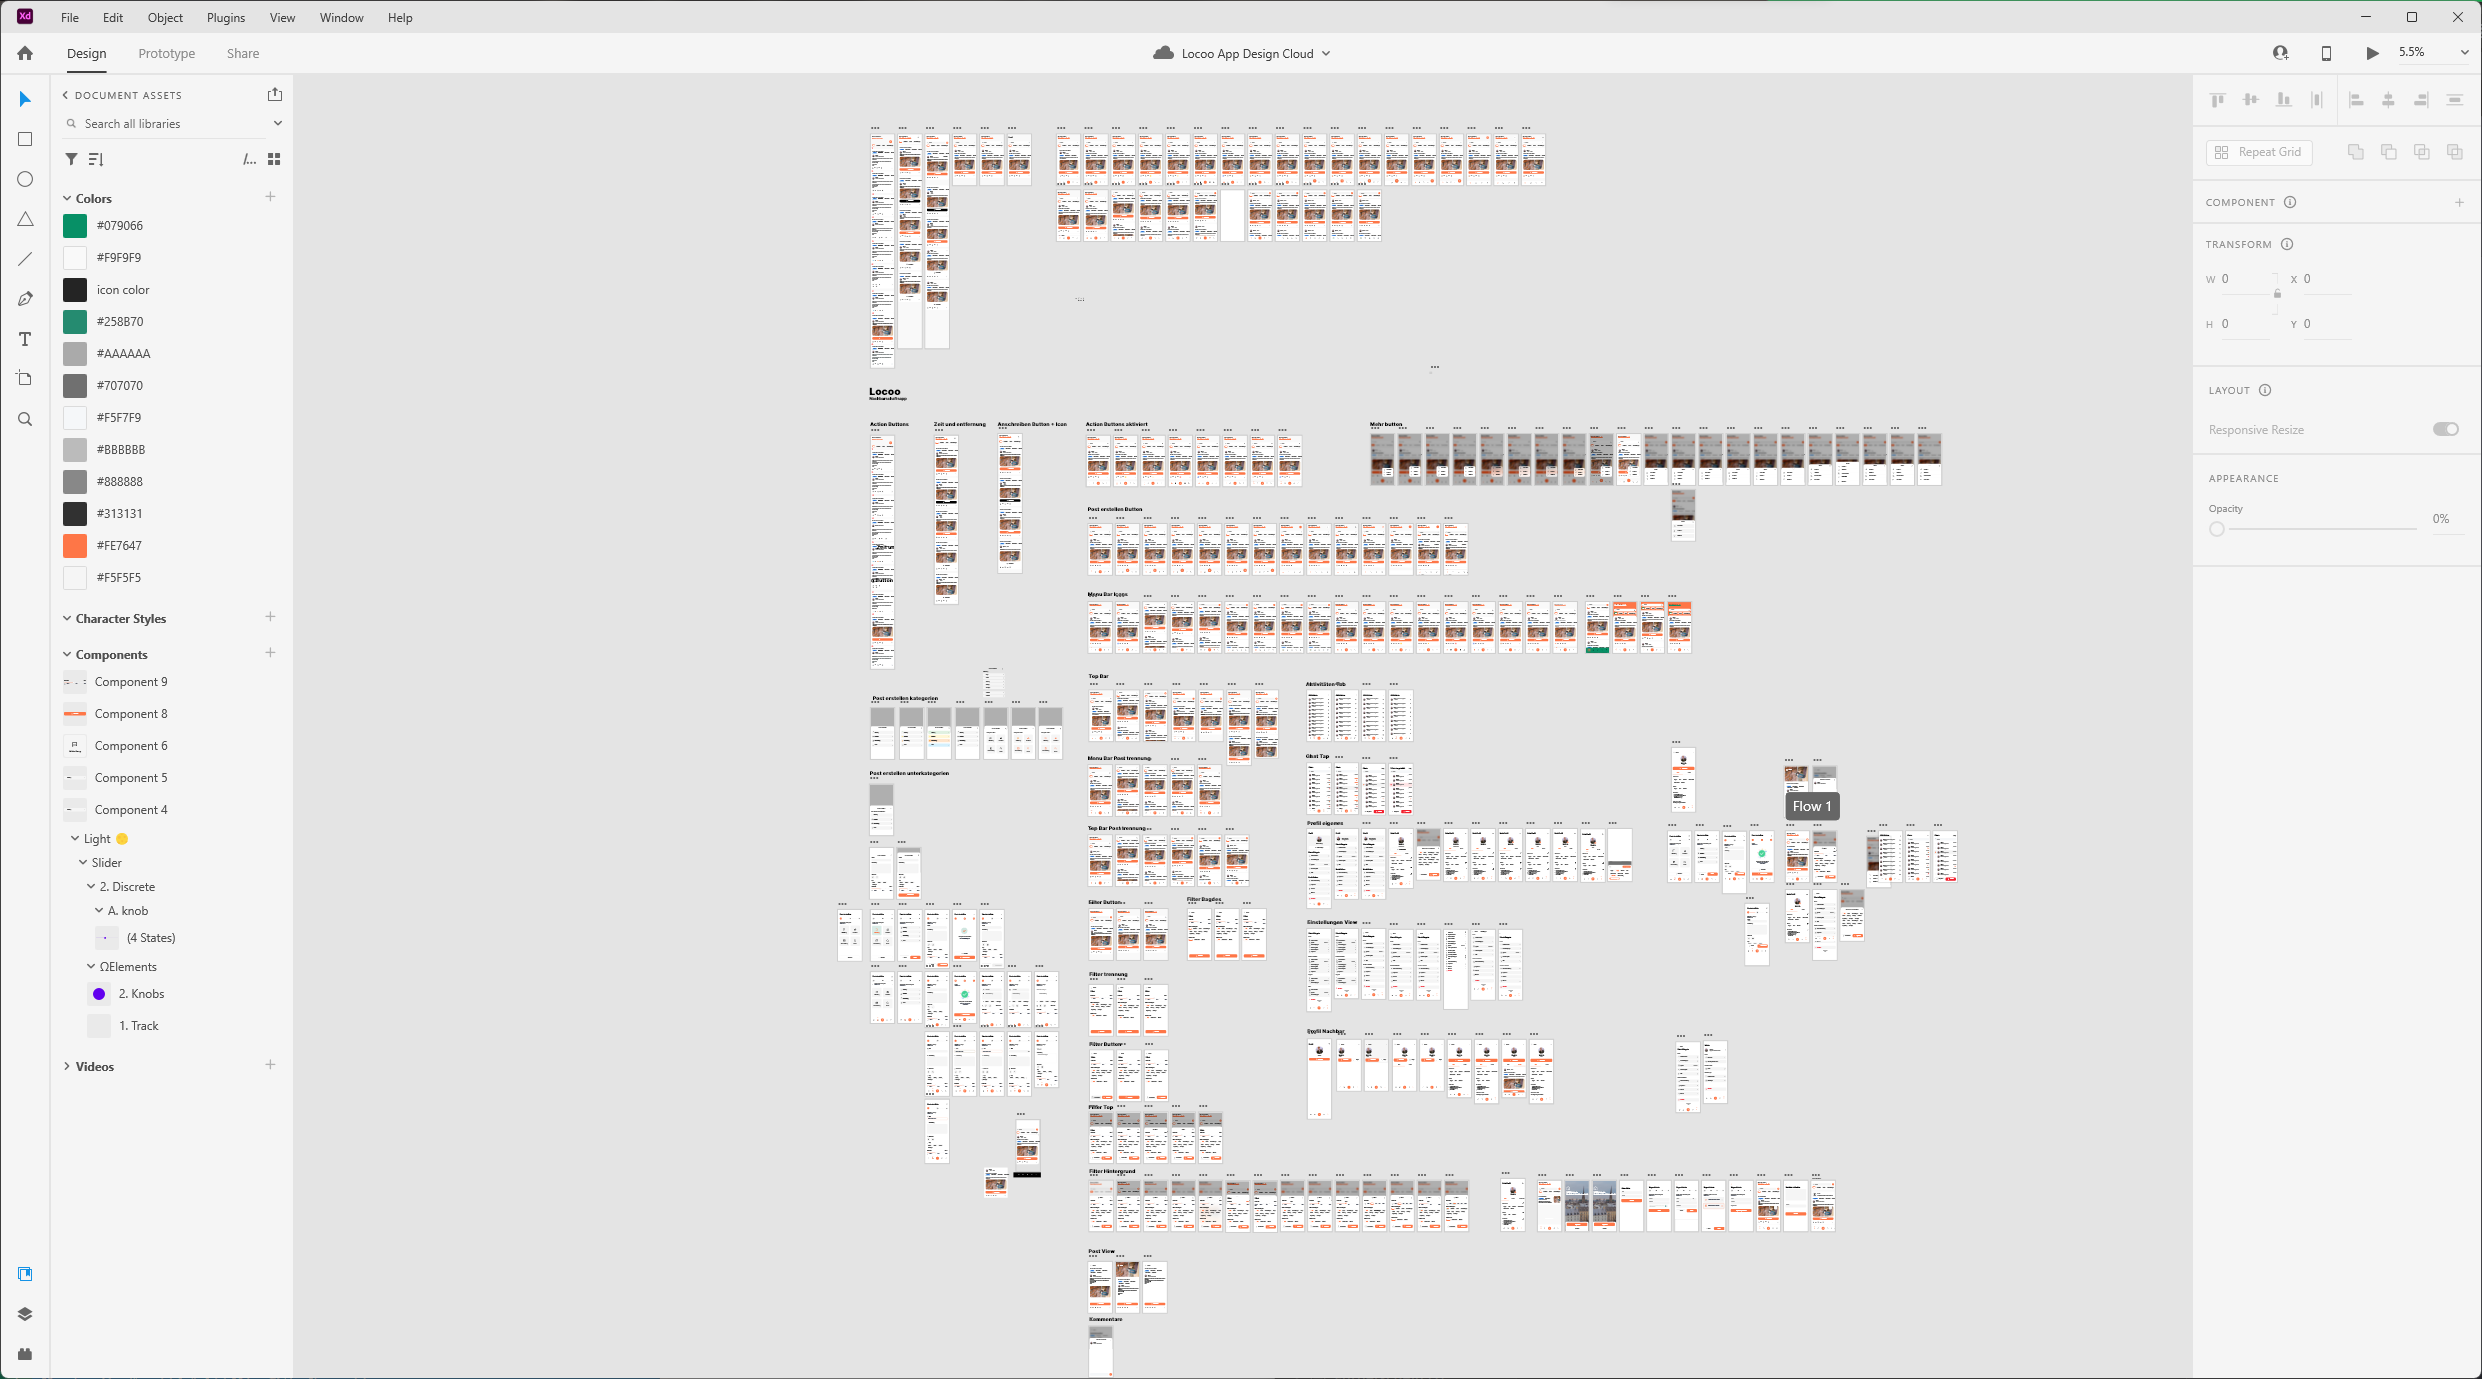
\includegraphics[width=0.95\textwidth]{pics/nochba-adobe-xd-protoype-screenshot.png}
  \caption{Nochba Prototyp in Adobe XD}
  \label{fig:adobexd-prototyp}
\end{figure}


Die Abbildung \ref{fig:adobexd-prototyp} zeigt eine
Sammlung von Designs und Designentwicklungen in unserem
Prototypen. Adobe XD war für unser Projekt geeignet, da
Martin Hausleitner als alleiniger Designer keine
Kollaborationsfunktion benötigte.

Jedoch ist der Designer mit
dem bekannteren und kostengünstigeren Figma vertraut, das
bei der Zusammenarbeit an einem Design und aufgrund der
zusätzlichen Funktionen besser geeignet ist.

Zusammenfassend kann festgestellt werden, dass Adobe XD ein leistungsstarkes Tool für UI/UX-Designer ist, das einfach zu bedienen ist und für kleine bis mittelgroße Projekte geeignet ist. Obwohl es nicht so viele Funktionen wie andere Tools bietet, eignet es sich gut für die schnelle Erstellung von Prototypen und eine einfache Zusammenarbeit mit Entwicklern und Stakeholdern.

\subsection{Design}
allg.

\subsubsection{Design System}
bild von allen componetns

\subsubsection{Farben}
Die Farbpalette einer Marke spielt eine wichtige Rolle im UI-Design, da sie dazu beiträgt, ein konsistentes Erscheinungsbild zu schaffen. Bei der Gestaltung einer Nachbarschafts-App wurde eine Vielzahl von Farbpaletten von anderen Apps untersucht. Es wurde festgestellt, dass die meisten großen Apps die Farbe Grün verwenden.

Obwohl Grün oft mit Natur und Gemeinschaft assoziiert wird, wurde sich bewusst dazu entschieden, sich von diesen etablierten Konventionen abzuheben. Stattdessen wurde die Farbe Orange ausgewählt, da sie auffällig und ungewöhnlich ist und somit das Potenzial hat, die App von anderen Nachbarschafts-Apps zu unterscheiden.

Zusätzlich passt die Farbe Orange gut zu den Werten der App, da sie für Wärme, Freundschaft und Optimismus steht - Eigenschaften, die in der App gefördert werden sollen. Die Hoffnung besteht darin, dass die Farbauswahl dazu beitragen wird, dass die Nutzer sich in der App wohl und willkommen fühlen und die Farbe sich als wiedererkennbares Markenzeichen etabliert.


\begin{figure}[h]
  \centering
  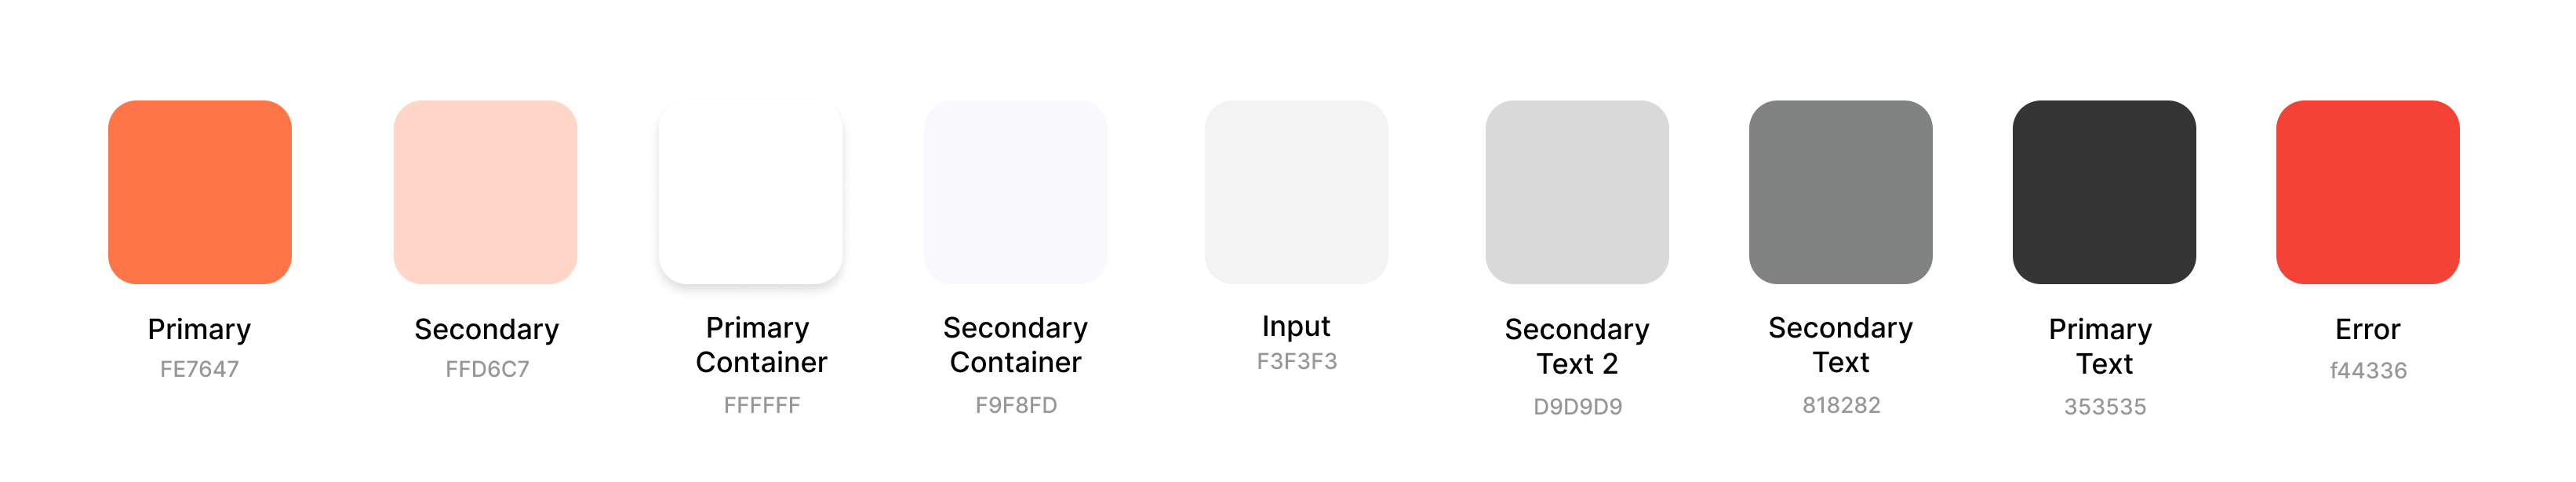
\includegraphics[width=1\textwidth]{pics/colors.png}
  \caption{Nochba Farbpalette}
  \label{fig:color-chart}
\end{figure}

Bevor der endgültige Farbton ausgewählt wurde, wurden verschiedene orangefarbene Töne für den Prototypen ausprobiert und für einige Tage beobachtet, um ein Gefühl für die Farbe zu bekommen. Schließlich wurde sich für die endgültigen Farben entschieden, wie in der Abbildung \ref{fig:color-chart} dargestellt.

Die Hauptcontainerfarbe für die meisten Ansichten ist Weiß, ebenso wie die Hintergrundfarbe der Posts. Allerdings wurde eine Farbe gesucht, die gut als Hintergrund passt, weshalb ein helles Grau verwendet wurde.

Für die Textfarbpalette wurde fast Schwarz gewählt, da dies zu einem weicheren Eindruck führt. Um Untertitel weniger präsent zu gestalten, wurde ein etwas hellerer Grauton gewählt.


\subsubsection{Icons}


\begin{figure}[ht]
  \centering
  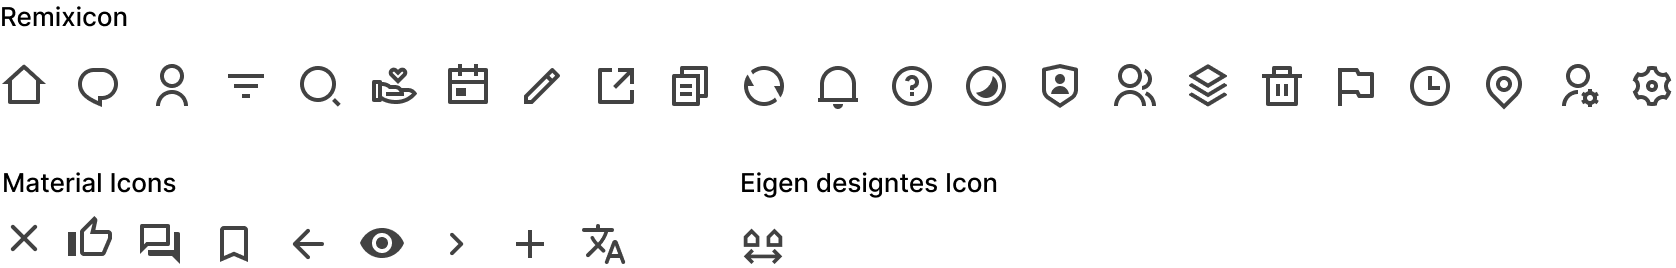
\includegraphics[width=1\textwidth]{pics/icons.png}
  \caption{App Icons}
  \label{fig:app-icons}
\end{figure}

Die obige Abbildung \ref{fig:app-icons} zeigt alle Icons,
die in einer App verwendet werden. Das Ziel war es, eine
möglichst große Anzahl von Icons zu integrieren, um die
Benutzerfreundlichkeit und Bedienbarkeit der App zu
verbessern. Nachdem verschiedene Icon-Packs betrachtet
wurden, wurde hauptsächlich das frei verfügbare
\href{https://github.com/Remix-Design/remixicon}{Remixicon}-Pack
verwendet, um der App ein einzigartiges Aussehen zu
verleihen und sie von anderen Apps abzuheben. Das runde
Design der Icons wurde besonders geschätzt. Ein weiterer
Vorteil von Remixicons ist, dass es ein
\href{https://pub.dev/packages/remixicon}{Flutter-Package}
gibt, was
die Implementierung erleichtert hat.

Obwohl Remixicons viele Icons zur Verfügung stellt, wurden
bei einigen Icons die
\href{https://fonts.google.com/icons?icon.set=Material+Icons}{Material Icons}
von Google bevorzugt.
Insbesondere die abgerundeten Icons wurden verwendet, um das
Design insgesamt weicher zu gestalten. Da kein passendes
Icon vorhanden war, um den Abstand zwischen zwei Nachbarn zu
symbolisieren, wurde ein neues Icon im Stil der anderen
entworfen.

\subsubsection{Typografie}
fotos von fonts
welche fonts
wie ist due typrographie aufgebaut
\subsubsection{Logo}

\begin{figure}[ht]
  \centering
  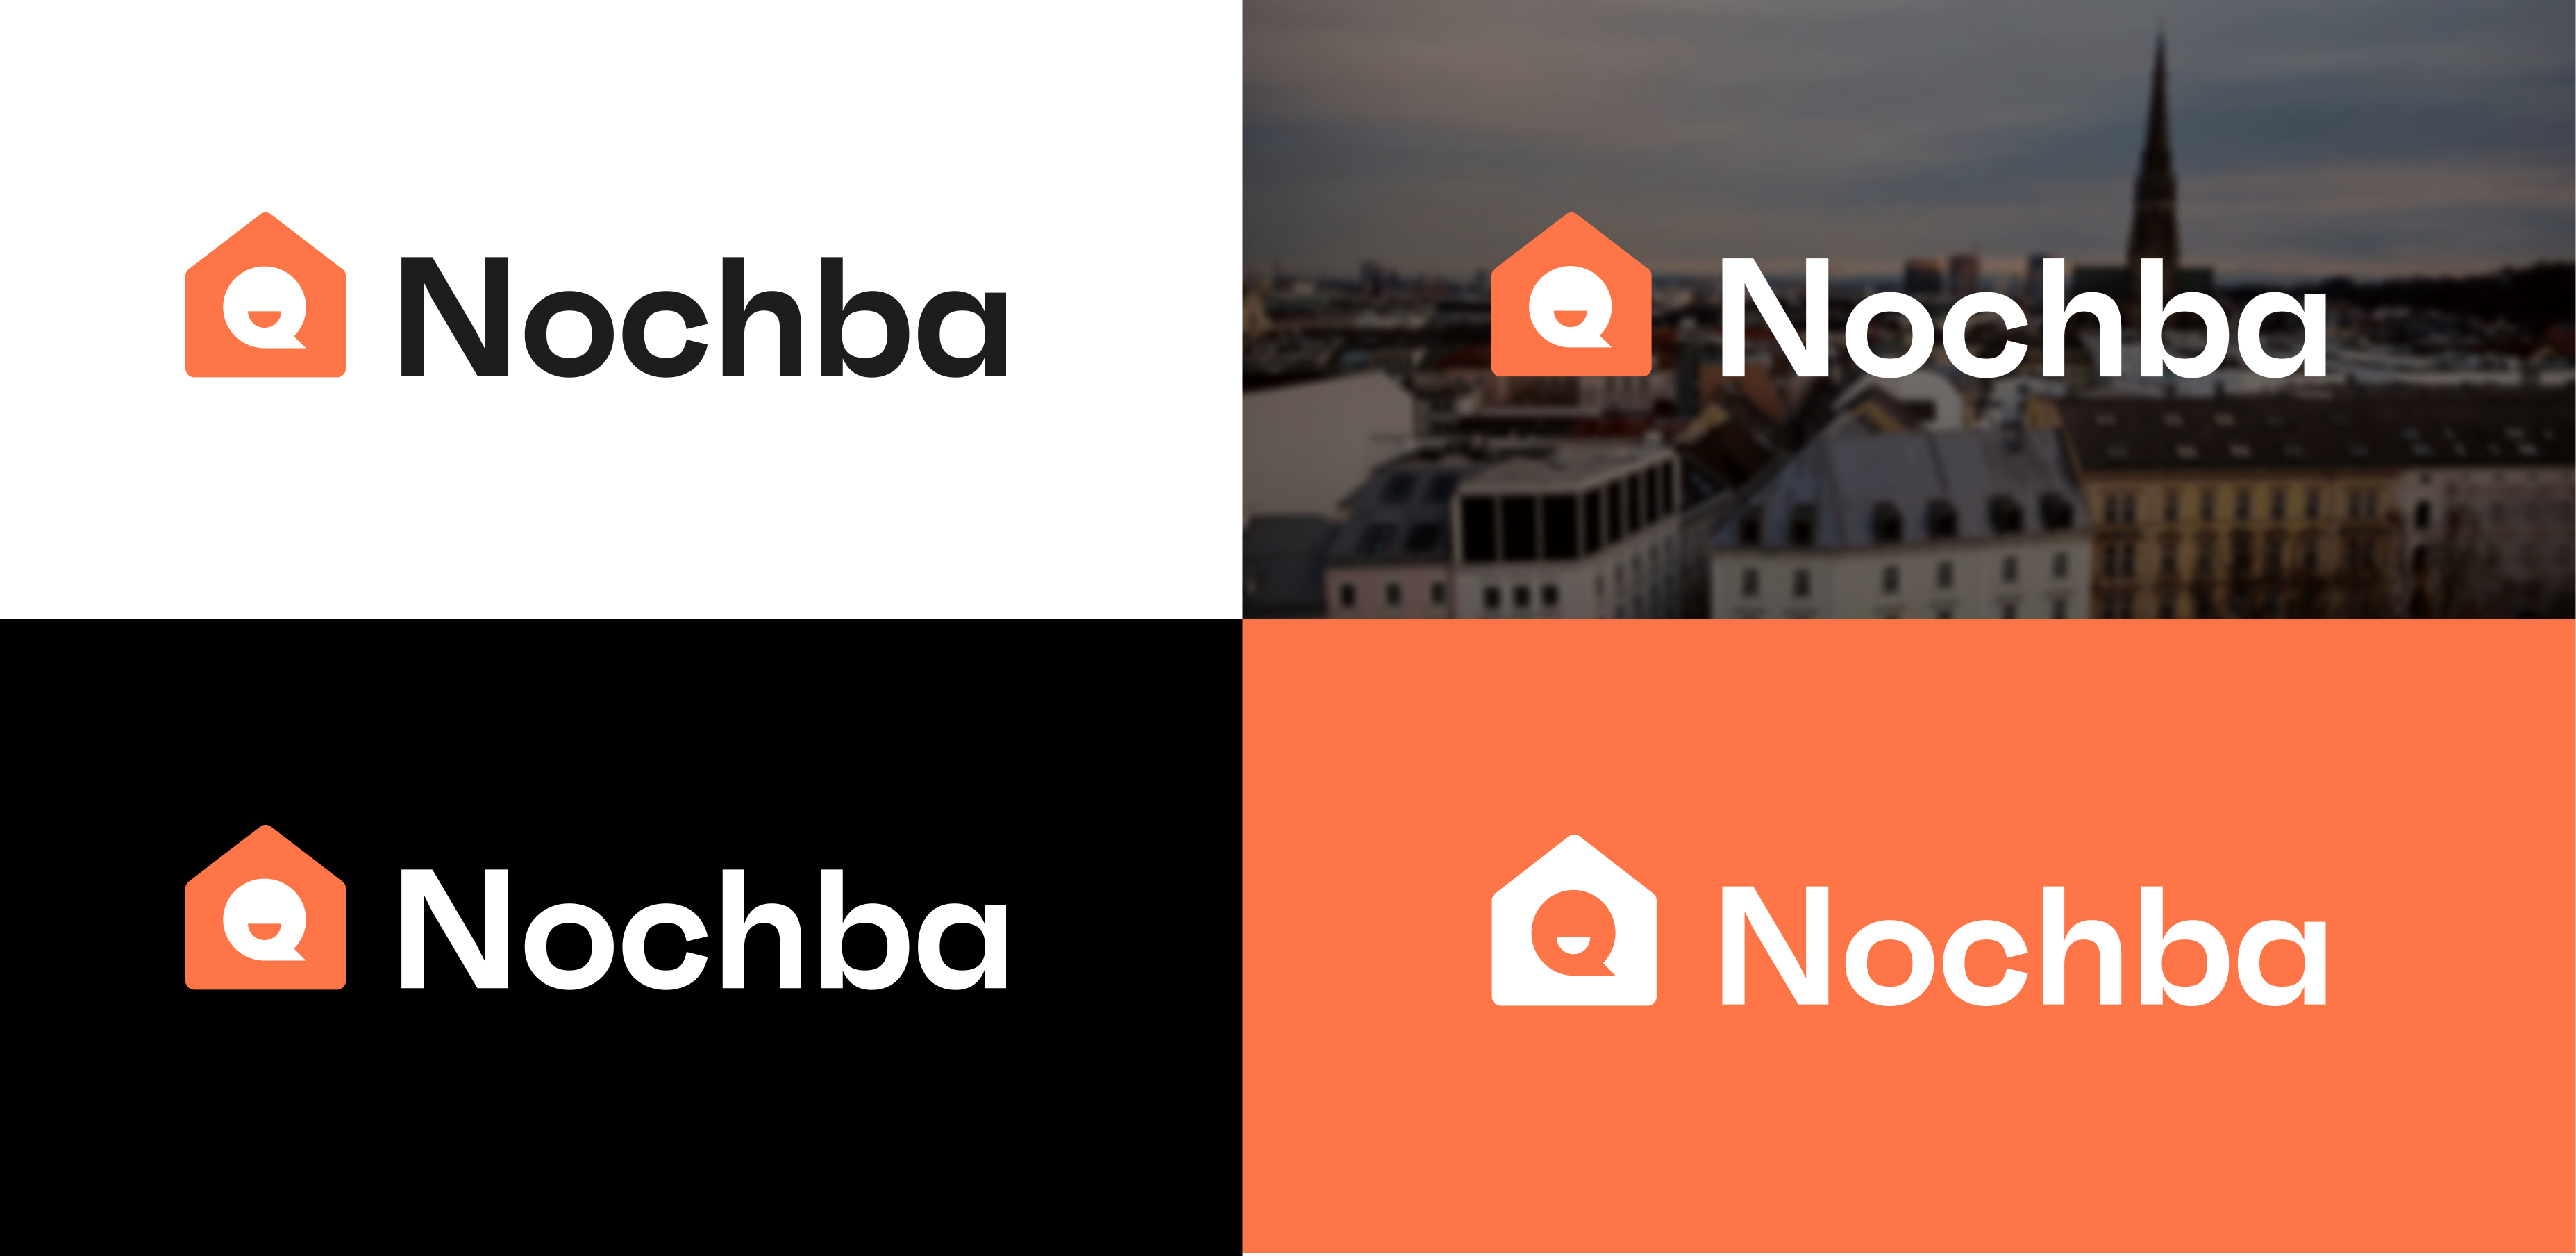
\includegraphics[width=0.95\textwidth]{pics/final-logo.png}
  \caption{Finales Logo}
  \label{fig:final-logo}
\end{figure}

% 
\includegraphics[width=0.35\textwidth]{pics/app-logo.png}

% überschrift logo historie
\paragraph{Logo Historie}

\begin{figure}[ht]
  \centering
  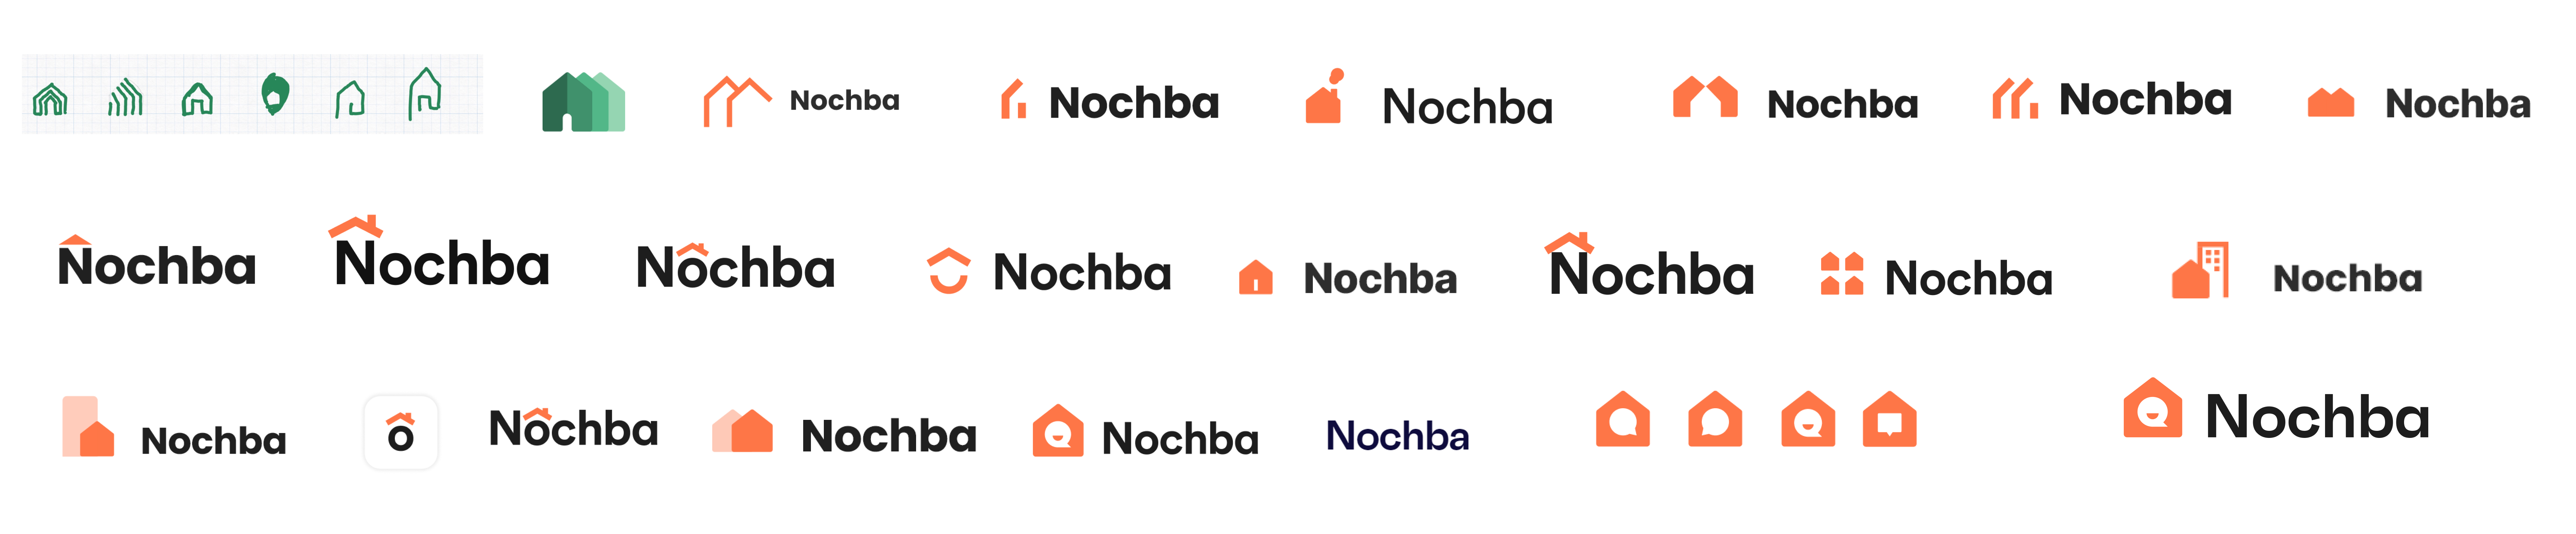
\includegraphics[width=0.95\textwidth]{pics/logo-historie.png}
  \caption{Logo Design Ideen}
  \label{fig:logo-historie}
\end{figure}

Im Zuge des Designprozesses wurden hohe Ansprüche an das
Logo der App gestellt, da es das Projekt repräsentiert und
es dem Team wichtig ist. Es
war wichtig, dass das Logo einfach gehalten und leicht
erkennbar ist. Die endgültige Gestaltung des Logos hat viel Zeit
in Anspruch genommen, da die vorherigen Entwürfe nicht
vollständig zufriedenstellten die man bei Abbildung
\ref{fig:logo-historie} sieht. Nach anderen Logos, die eine
Verbindung zu Nachbarschaften oder Häusern herstellen, wurde
gezielt gesucht und Ideen auf dem Discord-Server
gespeichert. Es sollte immer ein Haus erkennbar sein, da
Häuser schnell mit Nachbarschaften in Verbindung gebracht
werden.

In den früheren Versionen der App gab es Schwierigkeiten,
ein ansprechendes App-Icon zu gestalten, da kein
eigenständiges Icon vorhanden war. Aus diesem Grund wurde
entschieden, den Schriftzug und das App-Icon (Logo) separat
zu gestalten, wie es auch bei anderen Apps üblich ist. Das
endgültige Logo wurde erst Ende 2022 entworfen, da alle
anderen Designs nicht gefielen. Es wurde ein Haus mit einer
sprechenden Sprechblase, die lächelt, als Logo
wie bei Abbildung \ref{fig:final-logo} zu sehen ist gewählt. Dies soll symbolisieren, dass
man innerhalb des Hauses sprechen kann und das Lächeln soll
verdeutlichen, dass man Freude mit seinen Nachbarn teilen
kann. Eine runde, verspieltere Schriftart wurde bewusst
gewählt, da sie besser mit der Farbmischung harmoniert als
die vorherige Schriftart.



\subsection{App Design}
\subsubsection{Thumb Zone Prinzip}
\begin{figure}[h]
  \centering
  \begin{minipage}[b]{0.3\textwidth}
    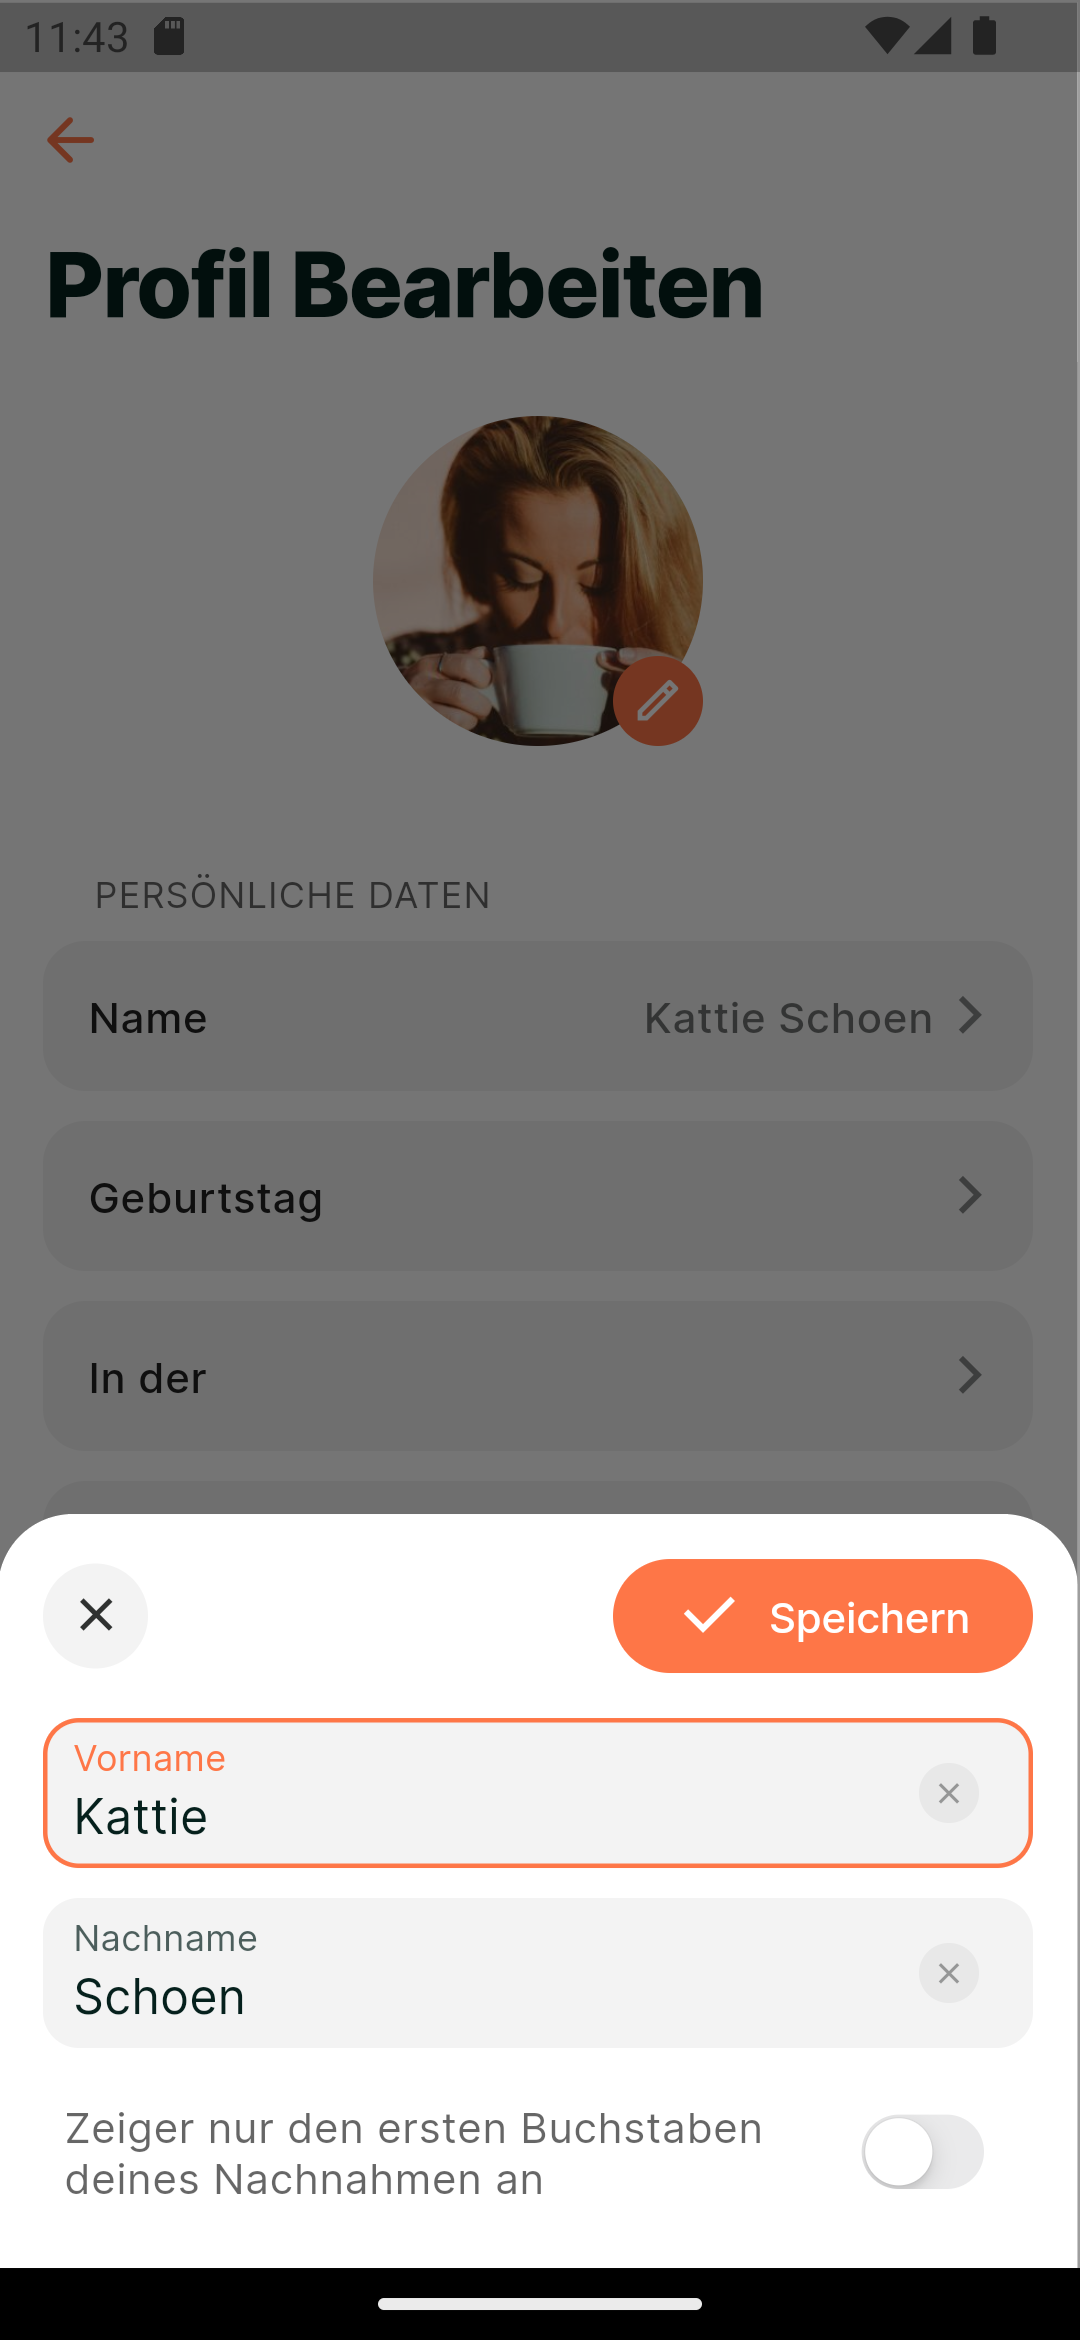
\includegraphics[width=\textwidth]{pics/edit-name-screen.png}
    \caption{Screenshot des "Name bearbeiten"-Screens}
    \label{fig:edit-name-screen}
  \end{minipage}
  \hfill
  \begin{minipage}[b]{0.3\textwidth}
    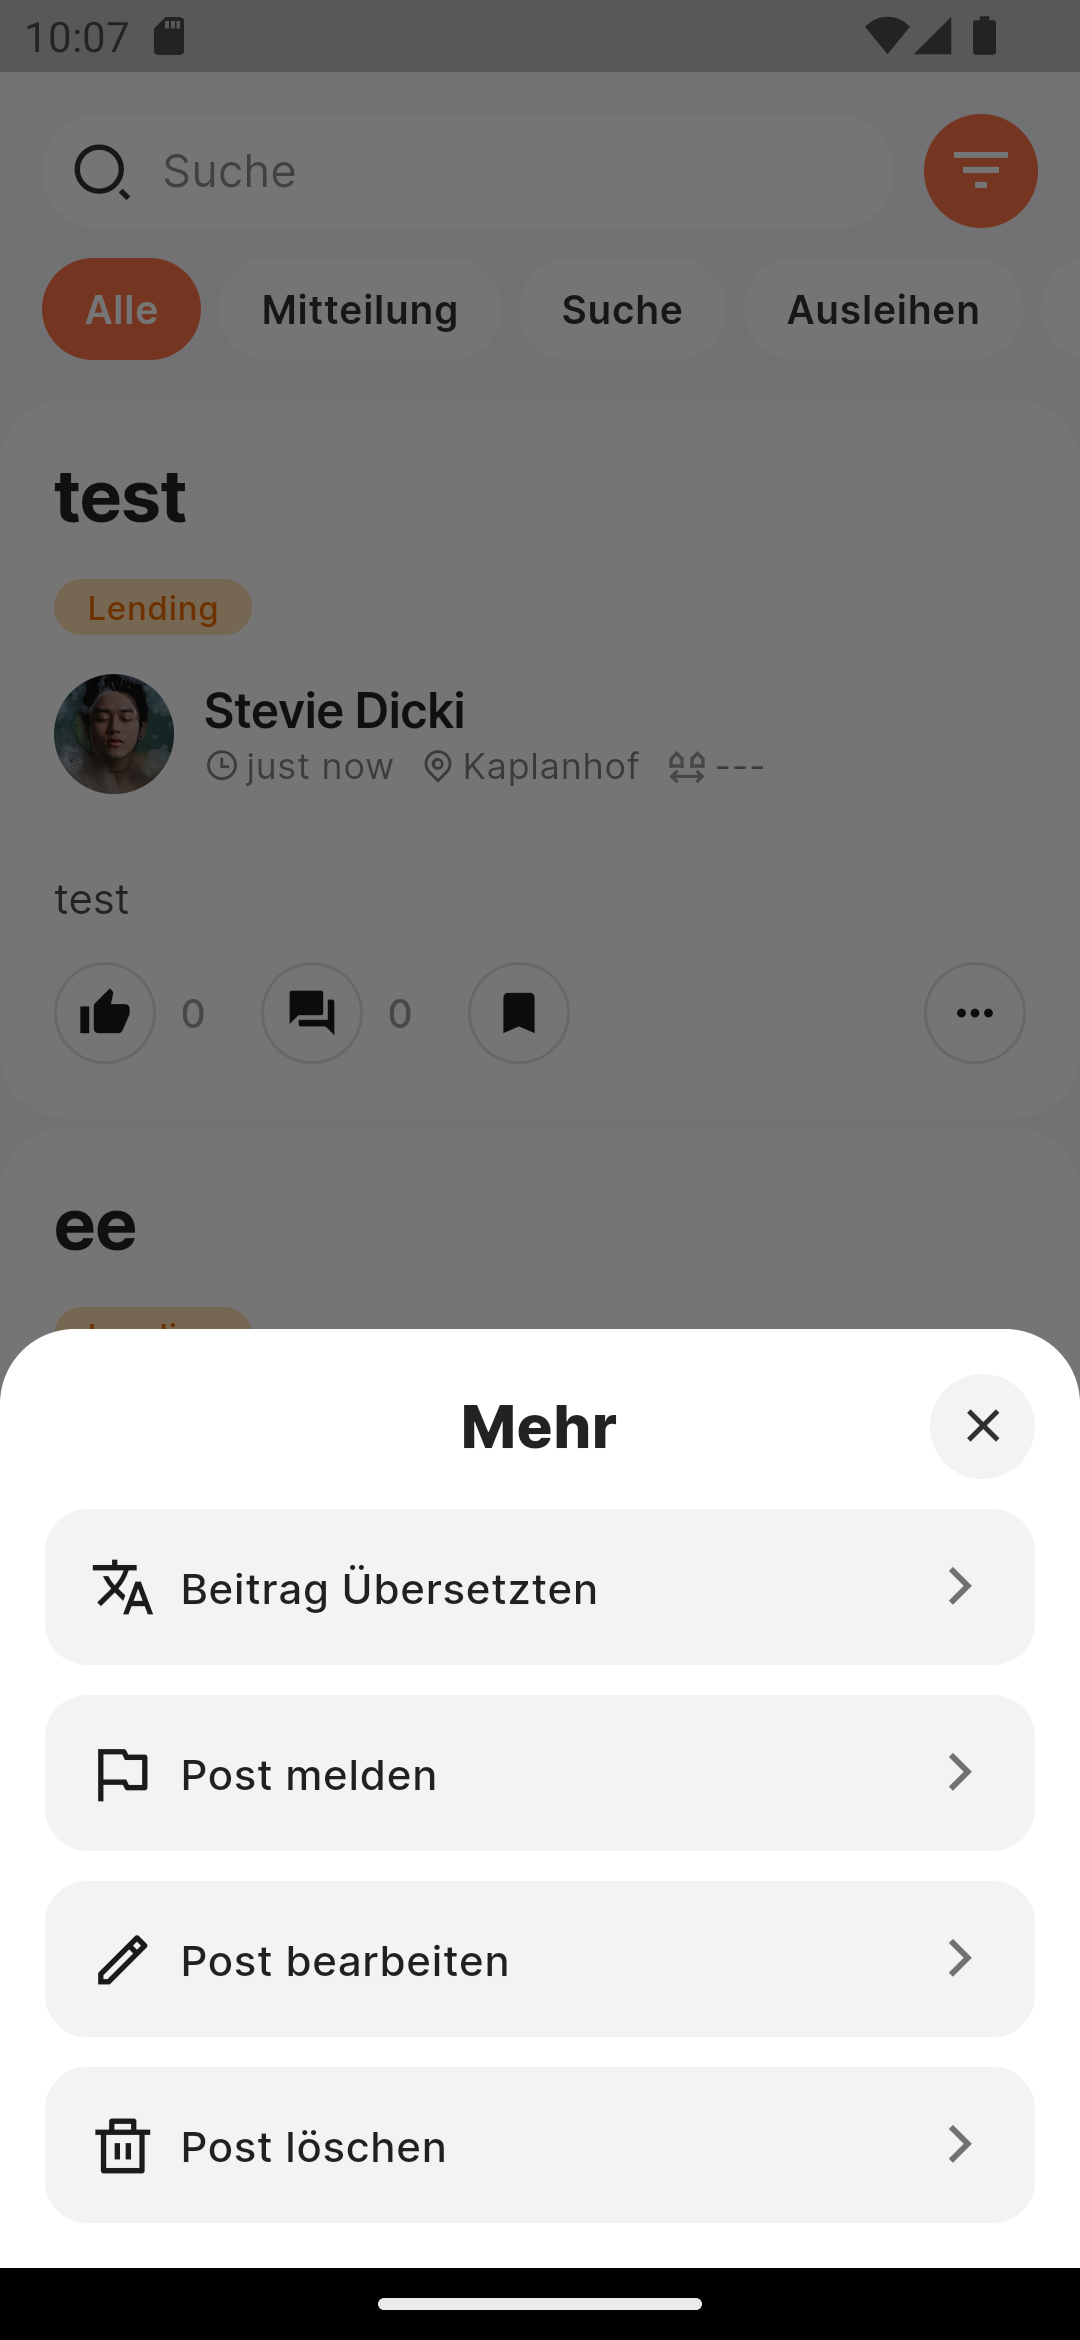
\includegraphics[width=\textwidth]{pics/post-more-menu.png}
    \caption{Screenshot des "Mehr"-Menüs für Beiträge}
    \label{fig:post-more-menu}
  \end{minipage}
  \hfill
  \begin{minipage}[b]{0.3\textwidth}
    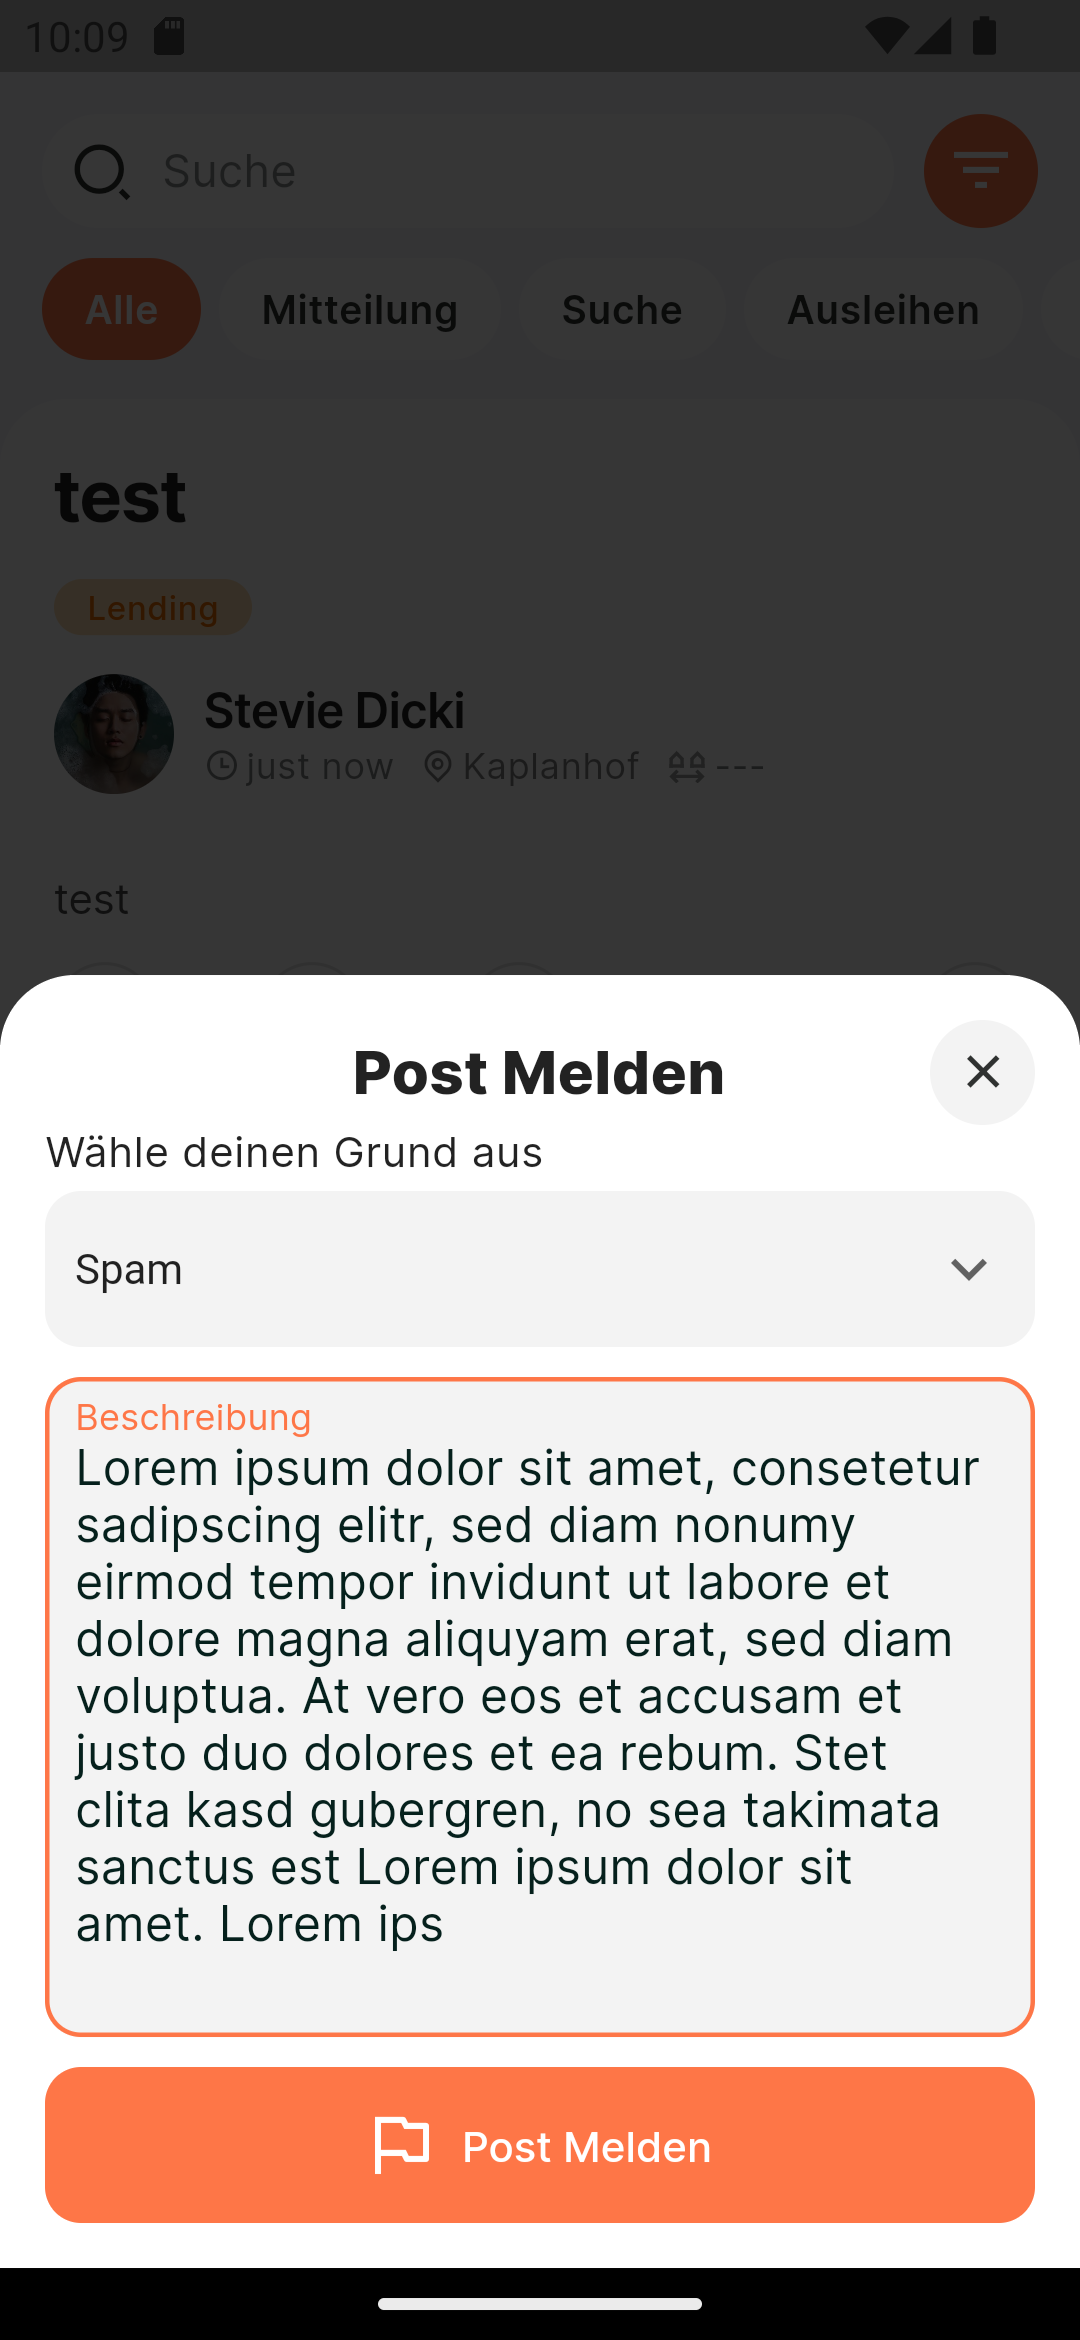
\includegraphics[width=\textwidth]{pics/post-report-menu.png}
    \caption{Screenshot des "Beitrag melden"-Menüs}
    \label{fig:post-report-menu}
  \end{minipage}
\end{figure}
Im Design-Muster wurde versucht, das Thumb Zone Prinzip zu
implementieren, indem wichtige UI-Elemente immer im unteren
Bereich der App platziert wurden. Das Layout für die
Namensbearbeitung \ref{fig:edit-name-screen} wurde extra
unten platziert, um alle Klick-Elemente bequem mit dem
Daumen bedienen zu können. Wichtige Buttons wie "Speichern"
wurden in der primären Farbe gestaltet und rechts
ausgerichtet, um einen leichteren Zugriff zu gewährleisten.
Das Textfeld kann einfach durch Drücken der Enter-Taste auf
der Tastatur geändert werden, um das Eintippen von Daten zu
erleichtern.

Wie bei Abbildung \ref{fig:post-more-menu} \ref{fig:post-report-menu} zu sehen ist, erfolgt eine weitere Implementierung einer Bottom View, um dem Thumb Zone Prinzip gerecht zu werden.

Unwichtige Buttons wurden in grau gestaltet, wie z.B. der X-Button in der Abbildung. Ein Löschen-Button neben dem Textfeld wurde eingebaut, der es dem Benutzer ermöglicht, den gesamten Text bequem zu löschen. Jedoch war es nicht möglich, diese Prinzipien vollständig umzusetzen, da die Zeit gegen Ende knapp wurde. In zukünftigen Versionen der App soll sichergestellt werden, dass diese Prinzipien einheitlich angewendet werden.
\subsubsection{Design Historie}

\begin{figure}[h]
  \centering
  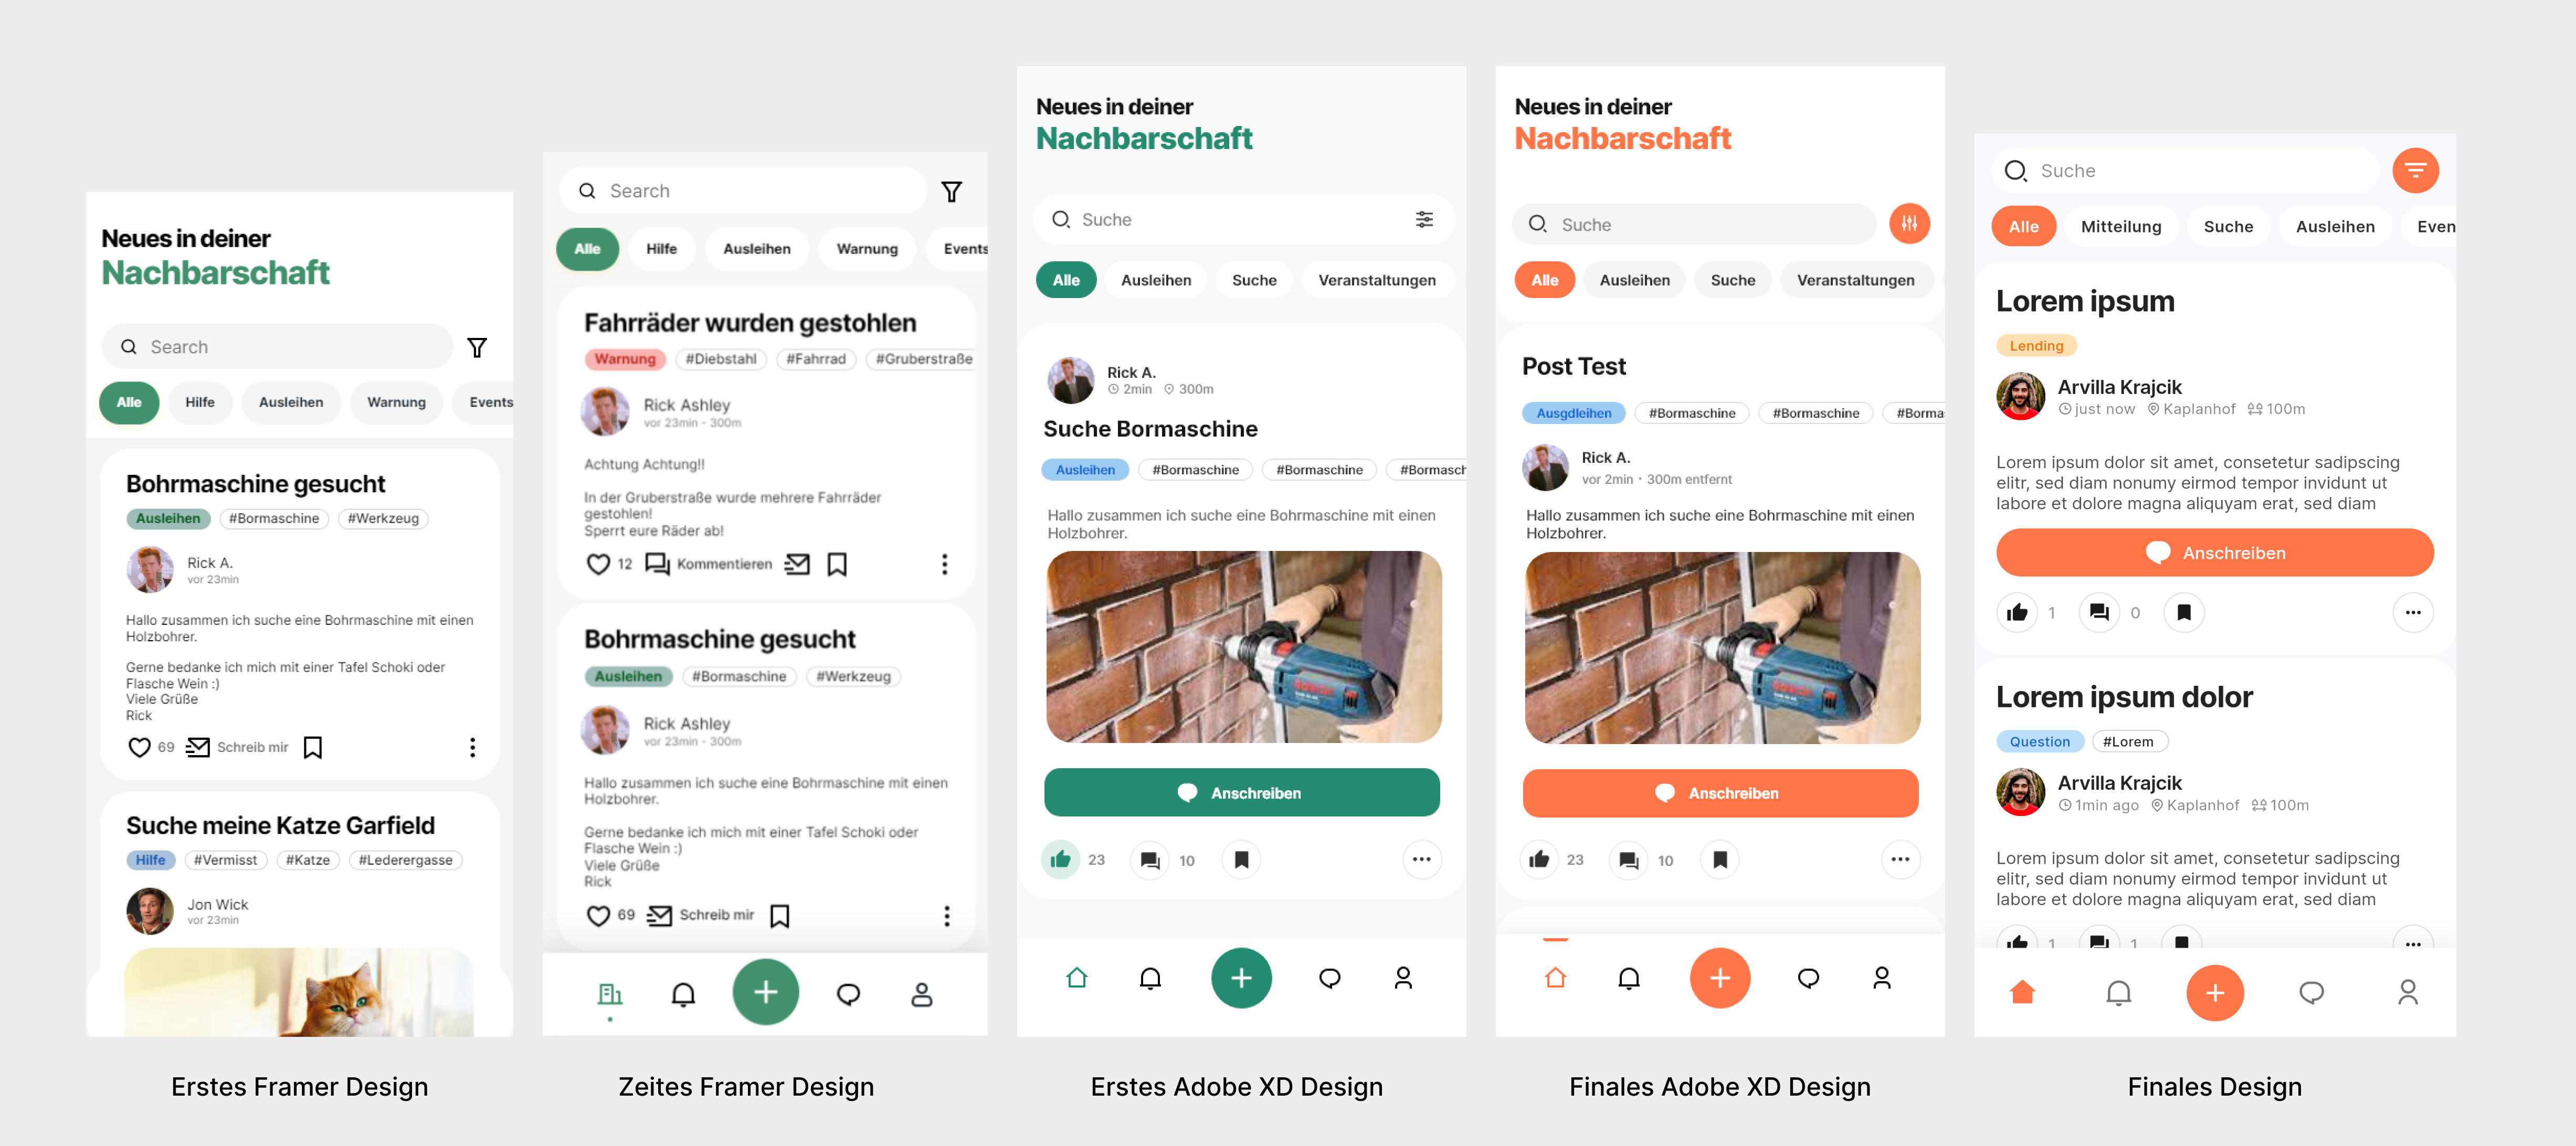
\includegraphics[width=1\textwidth]{pics/app-design-history.png}
  \caption{Screenshots verschiedener Versionen des App-Home-Screen}
  \label{fig:app-design-history}
\end{figure}
Im Rahmen des Hackathons Linz haCKt wurde das erste Design in Abbildung \ref{fig:app-design-history} ganz links erstellt. Hierbei wurden mehrere Brainstorming-Meetings mit Mentoren abgehalten, um ein Grundkonzept in Adobe XD zu gestalten. Anschließend wurden die groben Züge des Designs in Absprache mit dem Team festgelegt. Ein funktionsfähiger Prototyp wurde in Framer erstellt und am Tag der Endpräsentationen vorgestellt und verlinkt. Nach Linz haCKt wurde das zweite Design in Framer entwickelt.

Zwischen dem zweiten Framer-Design
\ref{fig:app-design-history} und dem ersten Adobe XD-Design
\ref{fig:app-design-history} wurde bewusst kein Abstand am
Rand eines Beitrags gehalten, um den vollen Handy-Display
auszunutzen. Der Filter-Button wurde mit der Suchleiste
verbunden, um das Design stimmiger zu gestalten. Bei den
Profilinformationen wurde auf Icons umgestellt, um es für
neue Nutzer verständlicher zu machen. Diese Entscheidung
wurde kurzzeitig verworfen, jedoch später in der Flutter-App
wieder eingebaut.

Wie man erkennen kann, wurde für das Finale Adobe
XD-Design \ref{fig:app-design-history} eine orangene Farbe für die Kapitelfarben
gewählt. Der letzte Screenshot zeigt die Flutter-App, wie
sie im Play Store erhältlich ist. Die größte Änderung
gegenüber dem vorherigen Design betrifft den Hintergrund
bei der Suche und der Kategorieauswahl. Der Hintergrund
wurde hellgrau gemacht, um die Beiträge besser hervorzuheben.
Bei der Entwicklung mit Flutter stellte sich heraus, dass
ein Strich über dem aktiven Icon sehr aufwändig zu
implementieren ist, weshalb darauf verzichtet wurde.



\section{Website}
\setauthor{Martin Hausleitner}
\begin{figure}[h]
  % \centering
  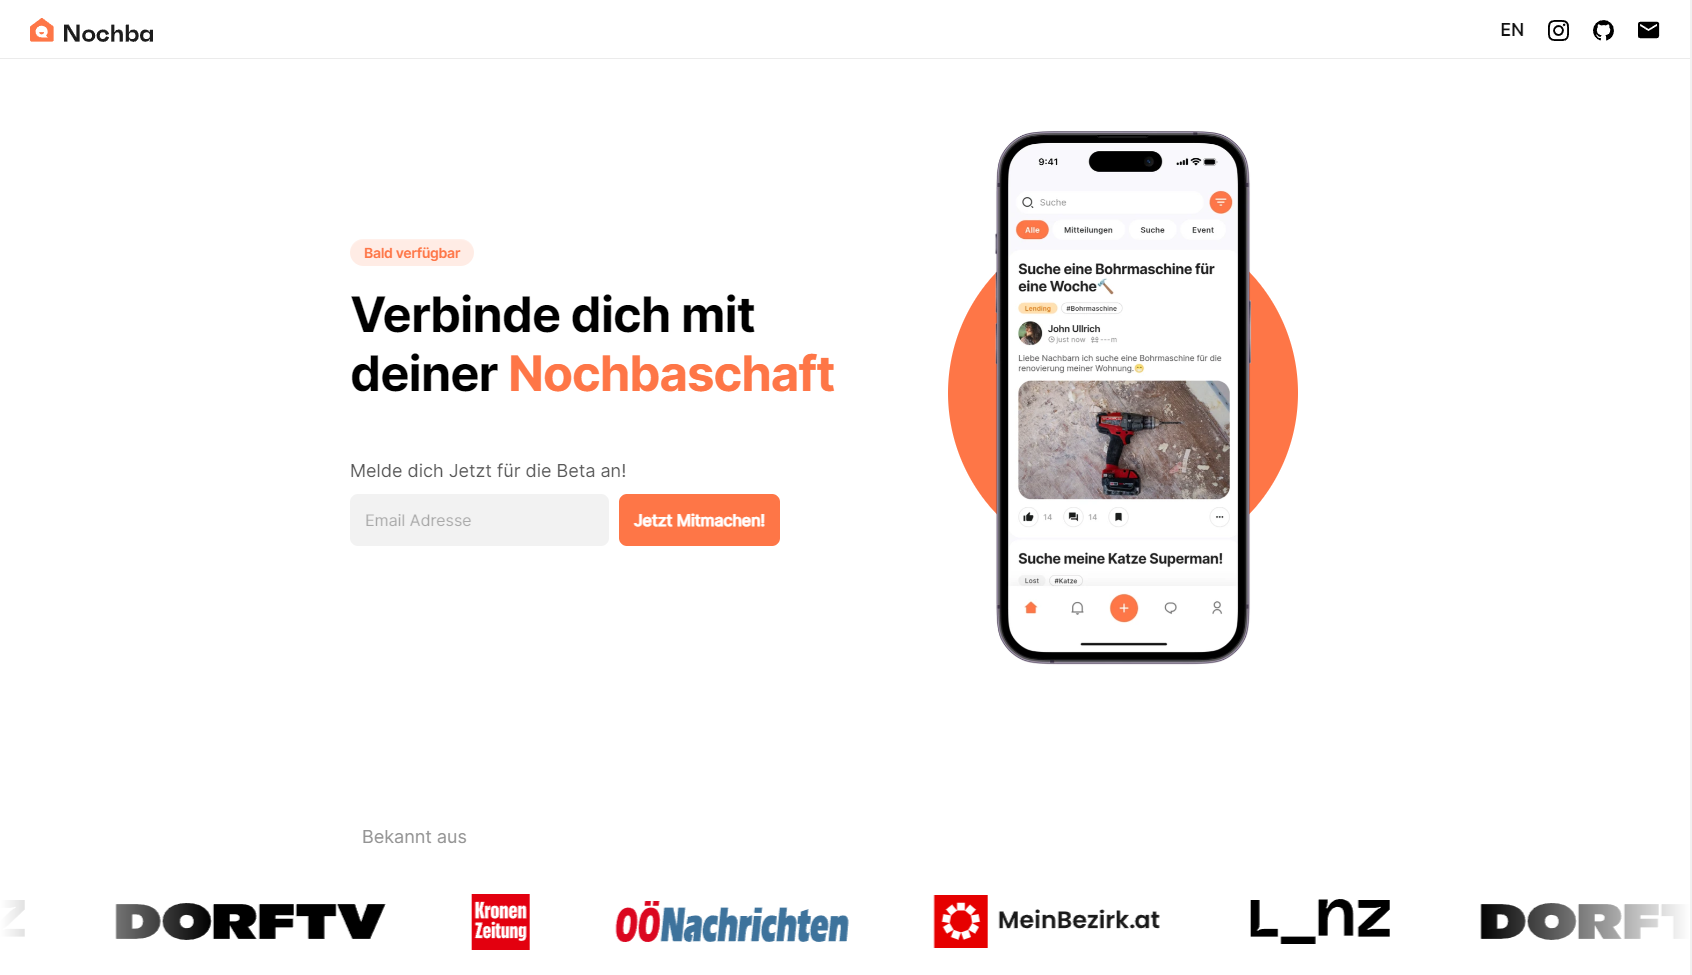
\includegraphics[width=1\textwidth]{pics/website-design.png}
  \caption{Screenshot der Nochba Website: nochba.at}
\end{figure}

Aufgrund der Medienpräsenz, die unser Projekt durch unsere Teilnahme an Linz hACkT erfahren hat und der Tatsache, dass wir keinen zentralen Anlaufpunkt für Informationen hatten, haben wir uns dazu entschlossen, eine schlichte Landing Page mit grundlegenden Informationen unter \href{https://nochba.at}{nochba.at} zu gestalten.

Unsere Teilnahme an dem mPreneur Social Mobile Entrepreneurship von Arsham Edalatkhah hat uns zu einer internationalen Aufmerksamkeit verholfen. Dies hat uns dazu bewogen, eine englischsprachige Website unter \href{https://nochba.com}{nochba.com} zu erstellen, um unsere Arbeit einem breiteren Publikum zugänglich zu machen und unsere Reichweite zu erhöhen.


\subsection{Beta-tester anmeldung}
Das wichtigste Merkmal der Website ist die Option für Nutzer, sich für die Testphase zu registrieren. Ursprünglich wurde versucht, die E-Mail-Adressen der Nutzer über die Google Sheets API zu speichern. Allerdings erwies sich dieser Ansatz als ineffektiv und dauerte mehrere Stunden. Als Alternative wurde das Framer-Add-On von Mailchimp.com genutzt, um Zeit zu sparen. Der kostenlose Plan von Mailchimp war für die Bedürfnisse ausreichend. Stand 7.3.2023 wurden 34 Beta-Anmeldungen über das Formularfeld gesammelt.


\subsection{Design}
Für die Gestaltung der Landing Page ließ sich der Designer
von den Vorlagen von Framer inspirieren und nutzte
vorgefertigte Abschnitte. Diese wurden jedoch so
modifiziert, dass sie dem Designsysten gerecht werden. Die
Farbpalette wurde beibehalten und es wurde darauf geachtet,
dass die Website möglichst einfach gestaltet ist.

\subsection{Kontent}
Auf der Website sind folgende Informationen abgebildet:
\begin{itemize}
  \item Zeitungsartikel
        \begin{itemize}
          \item \href{https://www.meinbezirk.at/linz/c-wirtschaft/linzer-nachwuchs-hacker-beweisen-sich-in-nordmazedonien_a5654095}{Mein Bezirk}
          \item \href{https://www.linz.at/medienservice/2022/202203_114704.php}{Linz}
          \item \href{https://www.nachrichten.at/oberoesterreich/linz/von-linz-nach-nordmazedonien;art66,3728292}{OÖNachrichten}
          \item \href{https://jugendhackt.org/video/nochba/}{DorfTV}
          \item Kronen Zeitung (nur auf Papier)
        \end{itemize}
  \item Unsere Mission
  \item Beitrag Kategorien
  \item Auszeichnungen
        \begin{itemize}
          \item Immotopia Innovation Award
          \item mPreneur Austria
          \item Linz hACkt
        \end{itemize}
  \item Features der App
  \item Partner der Diplomarbeit
  \item Über uns
  \item Links
        \begin{itemize}
          \item \href{https://github.com/Martin-Hausleitner/Nochba}{Github Repo}
          \item \href{https://www.instagram.com/nochba.at/}{Instagram}
          \item Email \href{mailto:project@nochba.com}{project@nochba.com}
        \end{itemize}
\end{itemize}


\subsection{Hosting}
Die Website wurde mithilfe von \href{https://framer.com}{Framer} erstellt und auf deren
Hosting-Plattform gehostet. Um die Domain-Namen zu nutzen,
die über \href{https://www.godaddy.com/de-at}{GoDaddy} (nochba.at und nochba.com) gekauft wurden, wurde eine Weiterleitung
mit Maskierung auf die entsprechende Framer-URL
eingerichtet. Durch diese Maßnahme wurde im Browser bei der
URL die gekaufte Domain angezeigt.

\subsubsection{SSL-Zertifikat}
Leider hat die Website derzeit kein SSL-Zertifikat, da durch
die Maskierung das Framer SSL-Zertifikat verloren geht.
Allerdings wird die Website im Browser nicht als bedrohlich
angezeigt, weshalb wir uns entschieden haben, kein
SSL-Zertifikat zu erstellen, um den Aufwand zu minimieren.

\section{Backend}

\subsection{Firebase}
\setauthor{Martin Hausleitner}
Firebase ist ein Backend-as-a-Service (BaaS), das Entwicklern eine enorme Erleichterung bei der Arbeit bietet. Das Hosting von Datenbanken und Cloud-Funktionen kann mit nur wenigen Klicks erfolgen, was die Notwendigkeit von Skalierung oder Ausfallvermeidung eliminiert. Das Firebase-Backend wird auf der Google Cloud in Frankfurt (EUR3 Europe-West) gehostet, um eine niedrige Latenz zu gewährleisten. Der kostenlose Spark-Plan war für den Gebrauch ausreichend, als der Dienst noch nicht die Firebase-Cloud-Funktionen genutzt hat. Um Kosten zu sparen, wurde lange Zeit mit dem Firebase-Emulator an den Cloud-Funktionen gearbeitet. Im Januar 2023 wurde auf den Blaze-Plan umgestiegen, um die Firebase-Cloud-Funktionen nutzen zu können. Bis März 2022 wurden nur wenige Euro für den Verbrauch gezahlt. Die Dokumentation und Tutorials von Firebase sind exzellent und es gibt viele Ressourcen auf YouTube.


\subsection{Firebase SDKs}
\setauthor{Sandin Habibovic}
Firebase SDK ist eine Sammlung von Software Development Kits, die von Firebase bereitgestellt werden, um Cloud-basierte Anwendungen zu erstellen.
Firebase SDK ist für eine Vielzahl von Programmiersprachen verfügbar, darunter JavaScript, Swift, Kotlin, Java und unter anderem Dart von Flutter.
Die Firebase SDK bietet eine breite Palette von Funktionen, mit denen leistungsstarke Anwendungen erstellt werden können, darunter Authentifizierung, Cloud Messaging, Cloud Firestore, Realtime Database, Cloud Functions. Mit diesen Funktionen können schnell und einfach Funktionen wie Benutzerverwaltung, Datenverwaltung, Messaging und Benachrichtigungen in Anwendungen integriert werden. Außerdem gibt es zu Firebase SDK eine umfangreiche Dokumentation und Support-Tools.

\subsection{Firebase Authentication}
\setauthor{Sandin Habibovic}
Email und Passwort authentication

\subsection{Cloud Firestore}
\setauthor{Sandin Habibovic}
NoSQL-Database, Dokument-basierte Speicherung, Subcollections
\subsection{Cloud Storage}
\setauthor{Sandin Habibovic}
Speicherung von Profilbilder und Post-Bilder
\subsection{Firebase Cloud Functions}
\setauthor{Martin Hausleitner}
Firebase Cloud Functions sind eine großartige Möglichkeit,
um Business-Logik abzubilden. Es handelt sich um serverlose
Funktionen, die in JavaScript oder TypeScript geschrieben
werden und einzeln auf der Google Cloud gehostet werden. Je
nach Nachfrage werden sie automatisch skaliert oder komplett
abgeschaltet. Ein Nachteil ist, dass die Startup-Zeit länger
sein kann als bei einem herkömmlichen Backend, das immer
läuft. Allerdings kann man durch Cloud Functions viel Geld
sparen, da nur die Prozessorlaufzeit bezahlt werden muss.

Firebase Cloud Functions ermöglichen es Entwicklern, auf verschiedene Ereignisse in Firebase-Produkten zu reagieren. Zum Beispiel, wenn sich Daten in der Firestore-Datenbank ändern oder ein neuer Nutzer in Firebase Authentication registriert wird. Wenn ein solches Ereignis eintritt, wird die entsprechende Cloud Function automatisch ausgeführt.

Wir haben alle Cloud Functions in TypeScript programmiert,
da es Typsicherheit und erweiterte Fehlererkennung
bietet.


\subsubsection{Regestrierung mit einen Verifizierungscode}
\setauthor{Martin Hausleitner}

Die Cloud-Funktion \texttt{checkVerificationCode} wird ausgeführt, wenn ein Nutzer sich mit einem Verifizierungscode registrieren möchte. Wenn der Benutzer nicht authentifiziert ist, wird eine \texttt{HttpsError} ausgelöst. Dann wird der Verifizierungscode überprüft, um sicherzustellen, dass er die korrekte Formatierung hat. Wenn der Code ungültig ist, wird eine weitere \texttt{HttpsError} ausgelöst.

Als Nächstes wird der Verifizierungscode mit der Datenbank abgeglichen, um sicherzustellen, dass er aktiv und noch nicht zu oft verwendet wurde. Wenn der Code erfolgreich validiert wird, wird die Adresse des Benutzers abgerufen und deren Koordinaten mithilfe einer API call an OpenStreetMap mit der Funktion \texttt{getOSMCoordinatesFromAddress} ermittelt. Dann wird die Entfernung zwischen der Adresse des Benutzers und der Adresse, die dem Verifizierungscode zugeordnet ist, berechnet mit der Funktion \texttt{getDistanceFromLatLonInMeters}. Wenn die Entfernung nicht innerhalb des zulässigen Bereichs liegt, wird eine weitere \texttt{HttpsError} ausgelöst.

Schließlich werden die Informationen des Benutzers und des Verifizierungscodes in der Datenbank aktualisiert, um anzuzeigen, dass der Benutzer erfolgreich verifiziert wurde. Die Cloud-Funktion gibt \texttt{true} zurück, um anzuzeigen, dass die Verifizierung erfolgreich war.

In jeder Phase der Funktion wird ein Logger verwendet, um Informationen über den Status der Funktion zu protokollieren.

\subsubsection{Regestrierung mit Gerät Koordinaten}
\setauthor{Martin Hausleitner}

Die Cloud-Funktion \texttt{checkAddressWithDeviceLocation} erfordert eine authentifizierte Anfrage und erhält eine Adresse sowie Längen- und Breitengradkoordinaten vom Gerät des Benutzers. Die Funktion prüft, ob alle erforderlichen Daten vorhanden sind und ruft dann die Funktion \texttt{getOSMCoordinatesFromAddress} auf, um die Koordinaten der angegebenen Adresse zu erhalten. Es wird auch die Funktion \texttt{getDistanceFromLatLonInMeters} aufgerufen, um die Entfernung zwischen der Adresse und den Koordinaten des Geräts des Benutzers zu berechnen.

Wenn die Entfernung größer ist als ein vordefinierter maximaler Abstand, wird eine Fehlermeldung ausgegeben und die Funktion gibt \texttt{false} zurück. Andernfalls speichert die Funktion die Koordinaten der Adresse und die Entfernung zwischen den Koordinaten des Geräts des Benutzers und der Adresse in der Firestore-Datenbank. Die Funktion ruft auch die Funktion \texttt{getOSMSuburbFromCoords} auf, um den Vorort der Adresse zu erhalten, und speichert diesen ebenfalls in der Firestore-Datenbank.

Die Funktion gibt \texttt{true} zurück, wenn die Verifizierung erfolgreich abgeschlossen ist.

In jeder Phase der Funktion wird ein Logger verwendet, um Informationen über den Status der Funktion zu protokollieren.

\subsubsection{Verifizierungscode generieren}
\setauthor{Martin Hausleitner}
Die Cloud-Funktion \texttt{generateVerificationCode} definiert Konstanten für das Intervall zwischen der Generierung von Codes, die maximale Anzahl von Codes und die Reichweite in Metern.

Anschließend wird der letzte Code des Nutzers aus der Datenbank geholt, um zu überprüfen, ob seit dem letzten generierten Code ausreichend Zeit vergangen ist. Wenn ja, wird der zuletzt generierte Code zurückgegeben.

Wenn nicht, wird eine Schleife gestartet, um einen neuen Code zu generieren mit der Funktion \texttt{generateRandomVerificationCode}. Der generierte Code wird dann mit Firestore abgeglichen, um sicherzustellen, dass er nicht bereits verwendet wurde.

Wenn der generierte Code eindeutig ist, wird überprüft, ob der Benutzer verifiziert ist. Wenn dies nicht der Fall ist, wird ein Fehler zurückgegeben. Andernfalls wird der generierte Code in die Firestore-Datenbank eingefügt, um den letzten generierten Code und das Datum der Generierung zu speichern.

Das Skript gibt dann den generierten Code zurück. In jeder Phase der Funktion wird ein Logger verwendet, um Informationen über den Status der Funktion zu protokollieren.

\subsubsection{Koordienaten von einer Adresse bestimmen}
\setauthor{Martin Hausleitner}
Ein wichtiger Teil für die Verifizierung ist, dass wir die Adresse des Nutzers in Koordinaten umwandeln, damit wir im Backend damit arbeiten können. Zunächst haben wir die Google Geocode API genutzt, allerdings kostet diese Geld. Wir haben eine bessere Option gefunden, die besser zu unserer Projekt-Philosophie passt: nämlich Nominatim, eine Open-Source-Geocoding-API für OpenStreetMap-Daten. Nominatim bietet eine kostenlose API für genau unser Problem an.

Die Funktion \texttt{getOSMCoordinatesFromAddress} nutzt die Bibliothek \texttt{axios}, um eine Anfrage an die Nominatim-API zu senden. Die API wird genutzt, um Koordinaten für eine Adresse zu erhalten.

Die Funktion nimmt einen Parameter \texttt{address} vom Typ \texttt{string} entgegen, welcher die Adresse enthält, für die Koordinaten abgerufen werden sollen.

Mithilfe von \texttt{axios.get} wird eine HTTP GET-Anfrage an die Nominatim-API gesendet. Die Adresse wird als URL-Parameter im Format \texttt{q=Adresse} übergeben. Die API liefert die Koordinaten als JSON-Objekt zurück, welches in der Variable \texttt{data} gespeichert wird.

Die Funktion überprüft dann, ob die Anfrage ein Ergebnis zurückgeliefert hat. Falls nicht, wird eine Fehlermeldung mit der Adresse ausgegeben.

Wenn ein Ergebnis vorhanden ist, wird das erste Ergebnis (in der Variable \texttt{firstResult}) verwendet, um eine neue Instanz der \texttt{GeoPoint}-Klasse zu erstellen. Diese Klasse ist Teil der Firebase-Admin-Bibliothek und ermöglicht die Speicherung von geografischen Koordinaten in einer Firestore-Datenbank.

\subsubsection{Entferung von zwei Nutzern berechnen}
\setauthor{Martin Hausleitner}
Die Cloud-Funktion \texttt{getDistanceFromTwoUsers} berechnet die Entfernung zwischen zwei Benutzern. Die Funktion erwartet eine \texttt{PostId} und einen authentifizierten Benutzer. Dann wird eine Überprüfung durchgeführt, ob der Post mit der angegebenen ID existiert und ob der Post eine gültige Reichweite hat. Es werden auch Überprüfungen durchgeführt, ob die Benutzerkoordinaten vorhanden sind, und ob die Entfernung zwischen beiden Benutzern innerhalb des Postbereichs liegt.

Die Funktion nutzt die importierten Funktionen \texttt{getDistanceFromLatLonInMeters} und \texttt{getNearestDistance}, um die Entfernung in Metern zu berechnen. Allerdings wird die berechnete Distanz grob gerundet, um die Privatsphäre der Nutzer zu wahren. Dabei werden die Längen- und Breitengradkoordinaten von zwei Benutzern miteinander verglichen, die aus der Firestore-Datenbank abgerufen werden. Wenn die Entfernung größer als die Reichweite des Posts ist, wird ein Fehler ausgegeben.

Schließlich gibt die Funktion die Entfernung zurück.

\subsubsection{Entfernung von zwei geographischen Koordinaten berechnen}
\setauthor{Martin Hausleitner}

\begin{lstlisting}[language=Java,caption=getDistanceFromLatLonInMeters Funktion]
    export function getDistanceFromLatLonInMeters(
        lat1: number,
        lon1: number,
        lat2: number,
        lon2: number
      ) {
        if (lat1 < -90 || lat1 > 90 || lon1 < -180 || lon1 > 180) {
          throw new Error(
            "Invalid coordinate: lat1 must be between -90 and 90, lon1 must be between -180 and 180"
          );
        }
        if (lat2 < -90 || lat2 > 90 || lon2 < -180 || lon2 > 180) {
          throw new Error(
            "Invalid coordinate: lat2 must be between -90 and 90, lon2 must be between -180 and 180"
          );
        }
        const R = 6371; // Radius der Erde in km
        const dLat = deg2rad(lat2 - lat1); // deg2rad unten
        const dLon = deg2rad(lon2 - lon1);
        const a =
          Math.sin(dLat / 2) * Math.sin(dLat / 2) +
          Math.cos(deg2rad(lat1)) *
            Math.cos(deg2rad(lat2)) *
            Math.sin(dLon / 2) *
            Math.sin(dLon / 2);
        const c = 2 * Math.atan2(Math.sqrt(a), Math.sqrt(1 - a));
        const d = R * c * 1000; // Distanz in Metern
      
        if (lat1 === lat2 && lon1 === lon2) return 0;
        return d;
      }
      
      function deg2rad(deg: number) {
        return deg * (Math.PI / 180);
      }
      
\end{lstlisting}
Der vorliegende Code implementiert eine Funktion, die die
Distanz in Metern zwischen zwei geographischen Koordinaten
(Breitengrad und Längengrad) auf der Erdoberfläche
berechnet. Die Funktion nutzt die Haversine-Formel, welche auf Kugelgeometrie basiert und aus der Quelle \cite{movabletype} movabletype in Javascript übernommen wurde, um die kürzeste Entfernung zwischen zwei Punkten auf der Erdoberfläche zu berechnen.

Die Funktion \texttt{getDistanceFromLatLonInMeters} hat vier Parameter: \texttt{lat1} und \texttt{lon1} sind die Breiten- und Längengrade des ersten Punktes, während \texttt{lat2} und \texttt{lon2} die Breiten- und Längengrade des zweiten Punktes sind, zwischen denen die Distanz berechnet werden soll.

Zu Beginn des Codes werden die Eingabeparameter auf ihre Gültigkeit geprüft und eine Fehlermeldung wird ausgegeben, falls eine der Koordinaten außerhalb des Bereichs von \texttt{-90} bis \texttt{90} für die Breite und \texttt{-180} bis \texttt{180} für die Länge liegt.

Die Funktion berechnet dann die Differenzen der Breiten- und Längengrade sowie den Radius der Erde (\texttt{R}) in Kilometern. Die Differenzen werden dann in Radianten umgewandelt und die Haversine-Formel wird angewendet, um die Entfernung in Kilometern zu berechnen. Schließlich wird das Ergebnis in Meter umgewandelt und zurückgegeben.

Die Funktion \texttt{deg2rad} wird als Hilfsfunktion definiert, um Grad in Radianten umzurechnen.

Die Funktion gibt \texttt{0} zurück, falls die beiden Eingabeparameter denselben Wert haben, um zu vermeiden, dass eine sehr kleine Distanz als Ergebnis ausgegeben wird, wenn es sich um denselben Punkt handelt.

Quelle: https://www.movable-type.co.uk/scripts/latlong.html

\subsubsection{Bestimmung der nächstgelegenen Entfernung}
\setauthor{Martin Hausleitner}
Um die Privatsphäre der Nachbarn zu gewährleisten, benötigen wir eine Funktion, die uns den nächstgelegenen Abstand zu den Nachbarn gibt, ohne den genauen Abstand preiszugeben. Die Funktion heißt \texttt{getNearestDistance} und bekommt einen Meterwert als Parameter.

Die Funktion erstellt ein Array mit den Optionen \texttt{[100, 200, 500, 1000, 5000, 10000, 15000]} und setzt die Variable \texttt{nearest} auf den ersten Wert im Array.

Dann wird eine Schleife ausgeführt, die durch jedes Element im Array \texttt{options} geht und prüft, welches Element am nächsten zum angegebenen Abstand \texttt{distance} liegt. Wenn ein Element näher ist als das bisher am nächsten liegende Element, wird \texttt{nearest} aktualisiert.

Schließlich wird überprüft, ob \texttt{nearest} größer oder gleich 1000 ist, und je nachdem wird der Abstand entweder in Kilometern oder Metern zurückgegeben. Wenn der Abstand größer oder gleich 1000 ist, wird die Einheit \texttt{km} hinzugefügt, ansonsten wird \texttt{m} hinzugefügt. Wir haben absichtlich keine Switches oder If-Bedingungen benutzt, da wir es jetzt mit der aktuellen Funktion schneller schaffen, die Abstände zu ändern. Wir evaluieren noch, wie das Array mit den Optionen aussieht.


\subsubsection{Nachbarschaft von Nutzer bestimmen}
\setauthor{Martin Hausleitner}
Um unseren App-Nutzern ein besseres Verständnis für die Nachbarschaften zu geben, in denen ihre Nachbarn wohnen, zeigen wir bei jedem Benutzer die Nachbarschaft an, in der sie leben. Diese Information wird automatisch in der Datenbank gespeichert, wenn der Nutzer verifiziert wird. Um diese Funktion zu ermöglichen, verwenden wir die folgende Funktion, die die geografischen Koordinaten des Benutzers verwendet, um die entsprechende Nachbarschaft mithilfe der OpenStreetMap-API abzurufen:

Die Funktion heißt \texttt{getOSMSuburbFromCoords} und nimmt zwei Parameter entgegen: \texttt{lat} für die geografische Breite und \texttt{lon} für die geografische Länge des Benutzers. Diese Funktion gibt eine Promise zurück, die eine Zeichenfolge \texttt{Stringn} mit dem Namen der Nachbarschaft des Benutzers enthält. Die Funktion verwendet die Axios-Bibliothek, um eine GET-Anfrage an die OpenStreetMap-API zu senden. Diese Anfrage enthält die geografischen Koordinaten des Benutzers und die gewünschte Zoomstufe \texttt{18}, um die Nachbarschaft zu finden. Wenn die Anfrage erfolgreich ist, gibt die Funktion den Namen der Nachbarschaft zurück, der aus den Daten extrahiert wird, die von der API zurückgegeben werden. Wenn der Name der Nachbarschaft nicht verfügbar ist, gibt die Funktion den Namen der Stadt oder der Gemeinde zurück, in der sich der Benutzer befindet. Wenn auch diese Informationen nicht verfügbar sind, gibt die Funktion \texttt{null} zurück. Wenn bei der Anfrage ein Fehler auftritt, wird eine Fehlermeldung ausgelöst.


\subsubsection{Verifizierungscode format überprüfen}
\setauthor{Martin Hausleitner}
Um die Laufzeit bei der Verifizierung von Cloud-Funktionen zu optimieren, ist es sinnvoll, am Anfang der Verifizierung eine Überprüfung durchzuführen, ob der Verifizierungscode das richtige Format hat. Dazu wird die Funktion \texttt{verifyVerificationCode} genutzt werden, welche einen \texttt{String} als Parameter erwartet und einen \texttt{Boolean}-Wert zurückgibt. In der Funktion wird ein regulärer Ausdruck Regex definiert, um sicherzustellen, dass der Verifizierungscode den Anforderungen entspricht. Der Regex lautet \texttt{/}\verb|^[a-zA-Z0-9]{10}$/|\texttt{,} was bedeutet, dass der Code aus genau 10 alphanumerischen Zeichen bestehen muss. Mit der Methode \texttt{checkVerificationCode} wird der übergebene Code auf Übereinstimmung mit dem Regex geprüft und das Ergebnis als \texttt{Boolean}-Wert zurückgegeben.

\subsubsection{Verifizierungscode generator}
\setauthor{Martin Hausleitner}

Die Funktion \texttt{generateRandomVerificationCode} erzeugt einen zufälligen Code mit einer Länge von 10 Zeichen, indem sie eine Kombination aus Groß- und Kleinbuchstaben des englischen Alphabets sowie Ziffern von 0 bis 9 verwendet. Dabei wird \texttt{Math.random()} zur Generierung einer Zufallszahl zwischen 0 und 1 genutzt und mit der Länge des Zeichenfolgen-Arrays multipliziert, um eine zufällige Position innerhalb des Arrays auszuwählen. Anschließend wird das ausgewählte Zeichen an das Ergebnis angehängt und dieser Schritt wird für jedes Zeichen wiederholt, bis eine Zeichenkette der Länge 10 generiert wurde.

Diese Funktion wird in der Cloud-Funktion \texttt{generateVerificationCode} verwendet, um einen zufälligen Code zu generieren. Es ist wichtig, dass der Code-Generator in der Lage ist, eine ausreichende Anzahl von Codes zu generieren, damit es keine Kollisionen gibt. Da jeder Code zufällig generiert wird und die Funktion eine zufällige Zeichenkette aus 62 möglichen Zeichen erzeugt, ist es äußerst unwahrscheinlich, dass der gleiche Code zweimal generiert wird. Die Anzahl der möglichen Kombinationen beträgt $62^{10}$, was ungefähr $8.39 \times 10^{17}$ Möglichkeiten entspricht. Daher ist die Wahrscheinlichkeit, dass zwei identische Codes generiert werden, vernachlässigbar.


\subsection{Algolia Search}
\subsection{Algolia SDK}

\subsubsection{Typesense Search}
\subsection{Typesense SDK}
